\documentclass[11pt,a4paper]{article}

\usepackage[margin=1in]{geometry}
\usepackage{amsmath,amssymb,amsthm,mathtools}
\usepackage{booktabs}
\usepackage{array}
\usepackage{microtype}
\usepackage{tikz}
\usetikzlibrary{arrows.meta,calc,decorations.markings,shapes.geometric}
\usepackage[colorlinks=true,linkcolor=blue!70!black,citecolor=red!70!black,urlcolor=blue!80!black]{hyperref}

% Typography & box control
\tolerance=3000
\emergencystretch=3em
\hfuzz=2pt
\hbadness=10000
\vfuzz=2pt
\vbadness=10000

\newtheorem{theorem}{Theorem}[section]
\newtheorem{proposition}[theorem]{Proposition}
\newtheorem{lemma}[theorem]{Lemma}
\newtheorem{corollary}[theorem]{Corollary}
\theoremstyle{definition}
\newtheorem{definition}[theorem]{Definition}
\newtheorem{remark}[theorem]{Remark}
\newtheorem{example}[theorem]{Example}
\newtheorem{observation}[theorem]{Numerical Observation}

\DeclareMathOperator{\Tr}{Tr}
\DeclareMathOperator{\spec}{spec}
\DeclareMathOperator{\diag}{diag}
\DeclareMathOperator{\rank}{rank}
\DeclareMathOperator{\Adj}{Adj}
\DeclareMathOperator{\Sym}{Sym}
\DeclareMathOperator{\Wg}{Wg}

\newcommand{\Q}{\mathbb{Q}}
\newcommand{\R}{\mathbb{R}}
\newcommand{\C}{\mathbb{C}}
\newcommand{\Z}{\mathbb{Z}}
\newcommand{\CF}{C_F}
\newcommand{\Ldn}{L_{\downarrow}}
\newcommand{\Lup}{L_{\uparrow}}
\newcommand{\Ssq}{S_{\square}}
\newcommand{\dg}{^{\dagger}}
\newcommand{\SU}{\mathrm{SU}}
\newcommand{\U}{\mathrm{U}}

% --- Disambiguated symbols (see the Notation table, Section 1.3) ---
\newcommand{\Bc}{\mathcal{B}}          % cellular coboundary matrix (was B(k))
\newcommand{\Rc}{\mathcal{R}}          % cross-plane hopping operator (was R)
\newcommand{\Utwo}{\mathcal{U}}        % two-hop cluster cumulant (was u(N))
\newcommand{\Ashp}{A_{\mathrm{shp}}}
\newcommand{\Bshp}{B_{\mathrm{shp}}}
\newcommand{\Cshp}{C_{\mathrm{shp}}}
\newcommand{\Dshp}{D_{\mathrm{shp}}}
\newcommand{\Wopp}{W_{\mathrm{opp}}}
\newcommand{\Wsame}{W_{\mathrm{same}}}

\title{\textbf{Homological Flat Bands, All-Rank Closed Forms, and the Hodge--Feshbach Decomposition in Strongly Coupled $\SU(N)$ Gauge Theory}}

\author{\textbf{Alexander Smith}\\[0.5em]
\small \textit{WORKHOUSE Theoretical Physics Research Group, Independent Research Initiative}\\[0.2em]
\small \texttt{alexander.smith.theory@gmail.com}}

\date{September 18, 2026\\[0.3em]\small Revision 2}

\begin{document}

\maketitle

\begin{abstract}
\noindent
We establish an exact correspondence between non-Abelian color dynamics and discrete cubical homology in the Hamiltonian formulation of strongly coupled $\SU(N)$ lattice gauge theory in three spatial dimensions. Restricting the Kogut--Susskind Hamiltonian to the fundamental, charge-odd one-plaquette shell, we prove seven theorems that determine the spectral geometry of the gauge field over the rational function field $\Q(N)$.

The second-order effective Hamiltonian on the fundamental plaquette shell factors exactly as $H_2 = t_N \Ldn = t_N \Bc\Bc\dg$, the tensor product of a universal color rational function $t_N = 2N(N^2-4)/[(N^2-1)(2N^2-1)(4N^2-9)]$ with the cellular down-Laplacian of the spatial 3-torus. Because $\partial_2\partial_3 = 0$, the spatial flux excitations are frozen into an exact flat band of macroscopic multiplicity $\dim\ker\partial_2 = (L^3-1)+3 = L^3+2$, spanned by $L^3-1$ compact localized states (elementary cube boundaries) and three non-contractible harmonic toron sheets generating $H_2(T^3;\R)$. The band is \emph{singular} in the sense of Rhim and Yang: the carrier eigenvector has no continuous limit at $\Gamma$, which is precisely why the compact states cannot span the carrier alone.

At fourth order, the Feshbach complement of the carrier is identically $\ker\Lup$, so neither Hodge Laplacian can leave the carrier and every excursion costs an insertion of the cross-plane operator $\Rc$. On the actual fourth-order operator support the carrier symbols span only $\{q,q^2,e_2\}$, which forces the two top-tier shape coefficients to vanish, $\Bshp = \Dshp = 0$. An audit of the fourth-order cluster expansion resolves a long-standing discrepancy: the adjacent-face cube completion requires all $24$ time-ordered insertion sequences, evaluating to $-53/768$, whereas historical series retained only $8$. Restoring the missing $16$ shifts the off-axis coefficient by $+25/1024$ and reconciles $\SU(3)$ with the all-rank formula with zero residual, showing the historical ``$\SU(3)$ exception'' to have been an enumeration defect. The resulting fourth-order dispersion $D_N(k) = \alpha_N\sum_i X_i^2 + \beta_N\sum_{i<j}X_iX_j$ has strictly positive rational coefficients for all $N\ge 3$, making $\Gamma$ the unique global band minimum and $(\pi,\pi,\pi)$ the unique global maximum.

Finally, the single-face holonomy class functions of $\U(N)$ map to $N$ non-interacting fermions in a Mathieu potential. Because the resulting one-body Hamiltonian has additive spectrum, the charge-parity splitting of the fundamental doublet is controlled by Mathieu band gaps at the Fermi surface and vanishes through order $N-2$; this is what makes the four intermediate irrep channels cancel at every even order and yields the grading law $S_m = O(N^{-(m+1)})$.

We are explicit about scope. Sections~\ref{sec:verification} and~\ref{sec:scope} separate what is proved unconditionally over $\Q(N)$, what is machine-checked in Lean~4 (three specific algebraic facts, not the full theorem list), and what is established numerically only --- notably a sharpening of the doublet result and the tower hypothesis (T) underlying the stronger $N^{-(2m-1)}$ grading law, which is \emph{not} proved here.
\end{abstract}

\newpage
\tableofcontents
\newpage

\section{Introduction and Summary of Main Theorems}\label{sec:intro}

\subsection{The Homological Gauge-Spectral Correspondence}

In condensed matter and photonic systems, flat bands---dispersion branches that remain strictly constant across the Brillouin zone---are engineered through fine-tuning of destructive interference in frustrated geometries such as kagome, Lieb, and line-graph lattices \cite{Sutherland1986,Lieb1989,Mielke1991,Tasaki1992,BergmanWuBalents2008,LeykamAndreanovFlach2018,Kollar2020}. Such bands host compact localized states (CLS) whose wavefunctions vanish identically outside a finite cluster.

We show that in strongly coupled non-Abelian gauge theory the same phenomenon arises without any tuning. Starting from the Kogut--Susskind Hamiltonian of pure $\SU(N)$ Yang--Mills theory on a spatial cubic lattice \cite{KogutSusskind1975}, the strong-coupling expansion of the lowest charge-conjugation-odd glueball states exhibits a flat band whose flatness is \emph{homological} rather than dynamical. The mechanism has two independent inputs:
\begin{itemize}\itemsep2pt
  \item \textbf{Color dynamics.} Non-Abelian Haar integration over the gauge link shared by adjacent plaquettes fixes the hopping amplitude via Weingarten calculus \cite{Weingarten1978,CollinsSniady2006}. This produces a single scalar $t_N \in \Q(N)$.
  \item \textbf{Cellular topology.} The interference signs between neighbouring plaquettes are fixed by the oriented boundary operator $\partial_2$ of the cubical complex of $T^3$ \cite{Eckmann1944,Dimakis1994,Forman1998}.
\end{itemize}
These combine into $H_2 = t_N \Ldn$ with $\Ldn = \partial_2\dg\partial_2$ the cellular down-Laplacian. Since $\partial_2\partial_3 = 0$, the boundary of every elementary $3$-cube is an exact zero mode: the flux excitations are frozen, and they are frozen for a reason that survives any change in the colour factor.

We emphasise at the outset what this is and is not. Every statement below concerns the strong-coupling expansion of a lattice Hamiltonian at finite lattice spacing, in a fixed low-lying sector. Nothing here is a statement about the continuum limit.

\subsection{Executive Overview of the Seven Theorems}

\begin{theorem}[Exact Tensor Factorization]\label{thm:intro_factorization}
Let $H_2$ be the second-order effective Kogut--Susskind Hamiltonian projected to the $3L^3$-dimensional charge-odd fundamental plaquette shell on $(\Z/L\Z)^3$. In the canonical basis of face orbitals $(p_1=(12), p_2=(13), p_3=(23))$ and link orbitals $(e_1,e_2,e_3)$, $H_2$ factors exactly as
\begin{equation}\label{eq:intro_H2}
  H_2 = E_{\mathrm{flat},N}\,I + t_N \, \Ldn, \qquad \Ldn = \Bc\Bc\dg,
\end{equation}
where $\Bc(k) = \partial_2(k)\dg = \begin{pmatrix} d_2 & -d_1 & 0 \\ d_3 & 0 & -d_1 \\ 0 & d_3 & -d_2 \end{pmatrix}$ with $d_j = e^{ik_j}-1$. The down-Laplacian satisfies $\Ldn(k) = q(k) I_3 - w(k)w(k)\dg$ with $w(k) = (\bar d_3, -\bar d_2, \bar d_1)^T$, and its Bloch spectrum is exactly $\{0, q(k), q(k)\}$ with $q(k) = 4\sum_{j}\sin^2(k_j/2)$.
\end{theorem}

\begin{theorem}[Topological Carrier Multiplicity]\label{thm:intro_multiplicity}
On a periodic cubic lattice of linear size $L\ge 3$,
\begin{equation}\label{eq:intro_dim}
  \dim \ker \partial_2 = (L^3 - 1) + 3 = L^3 + 2,
\end{equation}
decomposing into $L^3-1$ linearly independent compact localized states given by the oriented boundaries of elementary $3$-cells ($\operatorname{im}\partial_3$), and $3$ non-contractible harmonic toron sheets spanning $H_2(T^3;\R)\cong\R^3$.
\end{theorem}

\begin{theorem}[Universal All-Rank Hopping Coefficient]\label{thm:intro_tN}
For every $N\ge 3$ the colour dynamical factor is the positive rational function
\begin{equation}\label{eq:intro_tN}
  t_N = \frac{2N(N^2-4)}{(N^2-1)(2N^2-1)(4N^2-9)} \in \Q(N).
\end{equation}
In particular $t_2 = 0$ for $\SU(2)$ by pseudo-reality, $t_3 = 5/612$ in agreement with the 1989 series of Hamer \cite{Hamer1989}, and $t_N = \tfrac{1}{4N^3} - \tfrac{1}{16N^5} - \tfrac{77}{64N^7} - \tfrac{1021}{256N^9} + O(N^{-11})$.
\end{theorem}

\begin{theorem}[Hodge--Feshbach Decomposition and Tier Collapse]\label{thm:intro_hodge}
On each Bloch fiber with $q(k) \ne 0$ the plaquette space splits orthogonally as $\C^3 = \ker\Ldn \oplus \ker\Lup$ with $\Lup = \partial_3\partial_3\dg$, and the Feshbach complement of the carrier is identically $Q = P_{\ker\Lup}$. Consequently $Q\Ldn\psi = Q\Lup\psi = 0$: neither Hodge generator can leave the carrier, and every excursion requires an insertion of the cross-plane operator $\Rc$. On the actual fourth-order operator support $\mathcal{S}_4 = \{I,\Ssq,\Ssq^2,\Lup,\Rc\}$ the carrier symbols lie in $\operatorname{span}_\Q\{q,q^2,e_2\}$, so the two degree-three shape coefficients vanish identically:
\begin{equation}
  \Bshp = 0, \qquad \Dshp = 0 \quad (\text{tier collapse}).
\end{equation}
\end{theorem}

\begin{theorem}[Adjudication of a Historical Discrepancy]\label{thm:intro_adjudication}
The adjacent-face cube completion cluster possesses $24$ time-ordered insertion orderings summing to $-53/768$. Historical calculations retained only $8$ orderings (totalling $-31/1536$), omitting $16$ that contribute $\Delta\varrho = -25/512$. This shifts the off-axis coefficient by $\Delta\Cshp = +25/1024$, giving
\begin{equation}\label{eq:intro_cshp}
  \Cshp = C_{\mathrm{historical}} + \tfrac{25}{1024} = -\frac{13035490122347}{550663802582400} \approx -0.0236723048\ldots
\end{equation}
With this correction $\beta_3 = 8\Ashp + 16\Cshp = \frac{15644916262153}{34416487661400}$ equals the all-rank rational function $P_{17}(N^2)/[N R_{20}(N^2)]$ at $N=3$ with zero residual.
\end{theorem}

\begin{theorem}[All-Rank Dispersion Shape and Global Extrema]\label{thm:intro_dispersion}
At fourth order the flat band acquires the cubic-invariant dispersion
\begin{equation}\label{eq:intro_DN}
  D_N(k) = \alpha_N \sum_{i=1}^3 X_i^2 + \beta_N \sum_{i<j} X_i X_j, \qquad X_i = 1-\cos k_i = 2\sin^2(k_i/2),
\end{equation}
with strictly positive rational coefficients for all $N \ge 3$,
\begin{equation}
  \alpha_N = \frac{640}{N(N^2-1)^3}, \qquad \beta_N = \frac{P_{17}(N^2)}{N R_{20}(N^2)}.
\end{equation}
Hence $\Gamma = (0,0,0)$ is the unique global band minimum, $\mathrm{R} = (\pi,\pi,\pi)$ the unique global maximum, and the fourth-order bandwidth is $\Delta W_{4,N} = \alpha_N + \beta_N$.
\end{theorem}

\begin{theorem}[Single-Face Free-Fermion Theorem]\label{thm:intro_fermion}
Under the Weyl integration formula the class-function algebra of a single $\U(N)$ plaquette maps via the Vandermonde determinant to $N$ non-interacting spinless fermions on a circle with one-body Hamiltonian $h = p^2 + 2u\cos\theta$, and
\begin{equation}
  H_{\SU(N)} = H_{\U(N)} - \frac{P^2}{N}, \qquad P = \sum_{j=1}^N p_j .
\end{equation}
Because $H_{\U(N)}$ is a sum of one-body operators, its spectrum in the doublet sector is additive in two independent Mathieu pair labels, and the charge-parity splitting of $\{F,\bar F\}$ is controlled by the Fermi-surface band gap $e_A^+ - e_A^- = O(u^{N-1})$. Hence the Bloch operator on the model space $\{F,\bar F\}$ obeys
\begin{equation}
  K_m[F][\bar F] = 0 \qquad \text{for every } m \le N-2 .
\end{equation}
Consequently every intermediate channel's leading $N^{-(m-1)}$ coefficient equals its $\U(N)$ value; the four channels $(\mathbf{1},\Adj,\Sym^2,\Lambda^2)$ enter with weights $(-4,+2,+1,+1)2^{m/2-2}$ summing to zero at every even $m$, and the splitting is generated entirely by the centre-of-mass term $P^2/N$, giving the grading law $S_m = O(N^{-(m+1)})$.
\end{theorem}

\begin{remark}[What Theorem~\ref{thm:intro_fermion} does \emph{not} assert]\label{rem:intro_fermion_scope}
The sharper law $S_m = O(N^{-(2m-1)})$ recorded in the source ledger is \emph{not} established here. It requires the tower hypothesis (T) of Section~\ref{sec:fermion_status}, which is supported numerically but unproved. Only $S_m = O(N^{-(m+1)})$ follows from the argument given.
\end{remark}

\subsection{Notation}\label{sec:notation}

Several symbols in the earlier literature on this system carry more than one meaning; Table~\ref{tab:notation} fixes the conventions used throughout and flags the collisions we have removed. Readers comparing with earlier drafts should note in particular that the two degree-three shape coefficients (which vanish) and the fourth-order dispersion coefficients (which do not) were previously both written $B$.

\begin{table}[htbp]
\centering
\caption{Notation, with the symbol collisions removed in this revision.}\label{tab:notation}
\vspace{0.4em}
\small
\begin{tabular}{@{}llp{5.8cm}@{}}
\toprule
Symbol & Meaning & Note \\
\midrule
$\Bc(k)$ & cellular coboundary matrix $\partial_2(k)\dg$ & formerly $B(k)$ \\
$\Ashp,\Bshp,\Cshp,\Dshp$ & fourth-order shape-ansatz coefficients & $\Bshp=\Dshp=0$ (Thm.~\ref{thm:tier_collapse}) \\
$\alpha_N,\beta_N$ & fourth-order dispersion coefficients & $\alpha_N = 4\Ashp$, $\beta_N = 8\Ashp + 16\Cshp$ \\
$\Wopp,\Wsame$ & Weingarten channel sums & formerly $A_N$, $B_N$ \\
$\Rc$ & cross-plane hopping operator & formerly $R$ \\
$\mathrm{R}$ & Brillouin-zone corner $(\pi,\pi,\pi)$ & distinct from $\Rc$ and $R_{20}$ \\
$u$ & strong-coupling coordinate $\beta_N/(2N)$ & \\
$\Utwo(N)$ & two-hop cluster cumulant & formerly also written $u(N)$ \\
$\varrho$ & adjacent-cube cluster weight & distinct from an irrep $\rho$ \\
$\tilde E^a_\ell$ & right-invariant electric field & formerly $R^a_\ell$ \\
$a_i,\;X_i$ & $4\sin^2(k_i/2)$, $\;2\sin^2(k_i/2)$ & $a_i = 2X_i$; see \eqref{eq:dictionary} \\
\bottomrule
\end{tabular}
\end{table}

The two families of symmetric coordinates are related by
\begin{equation}\label{eq:dictionary}
  a_i = 2X_i, \qquad q = \sum_i a_i = 2\sum_i X_i, \qquad e_2 = \sum_{i<j}a_ia_j = 4\sum_{i<j}X_iX_j,
\end{equation}
which is the dictionary converting the operator-basis results of Section~\ref{sec:hodge} into the dispersion of Section~\ref{sec:dispersion}. Explicitly, the shape ansatz term $\Ashp q^2 + 4\Cshp e_2$ becomes $4\Ashp\sum_i X_i^2 + (8\Ashp + 16\Cshp)\sum_{i<j}X_iX_j$, which is the origin of the identifications $\alpha_N = 4\Ashp$ and $\beta_N = 8\Ashp + 16\Cshp$ recorded in Table~\ref{tab:notation}.

\section{Hamiltonian Lattice Gauge Theory and the Plaquette Shell}\label{sec:hamiltonian}

\subsection{Kogut--Susskind Formulation}

We consider pure $\SU(N)$ lattice gauge theory in continuous time on a three-dimensional cubic spatial lattice $\Lambda = (\Z/L\Z)^3$ with lattice spacing $a=1$ and periodic boundary conditions, $L\ge 3$. To each oriented spatial link $\ell = (x,\mu)$, $\mu\in\{1,2,3\}$, is assigned $U_\ell \in \SU(N)$. The Hilbert space is $\mathcal{H} = \bigotimes_\ell L^2(\SU(N), dU_\ell)$ with $dU_\ell$ the normalized Haar measure.

The Kogut--Susskind Hamiltonian \cite{KogutSusskind1975} in electric units is
\begin{equation}\label{eq:H_KS}
  H = H_E - u V, \qquad
  H_E = \frac{1}{2}\sum_\ell \sum_{a=1}^{N^2-1}(E^a_\ell)^2, \qquad
  V = \sum_p\left(\Tr U_p + \Tr U_p\dg\right),
\end{equation}
where $E^a_\ell$ are left-invariant Lie algebra generators satisfying $[E^a_\ell, E^b_{\ell'}] = i f^{abc}E^c_\ell \delta_{\ell\ell'}$, and $U_p = U_{x,\mu}U_{x+\hat\mu,\nu}U\dg_{x+\hat\nu,\mu}U\dg_{x,\nu}$ is the path-ordered holonomy around the elementary plaquette $p = (x,\mu<\nu)$. The parameter
\begin{equation}\label{eq:u_def}
  u = \frac{\beta_N}{2N} = \frac{1}{g_H^4}
\end{equation}
is the all-rank strong-coupling coordinate, which coincides with $\beta_3/6$ for $\SU(3)$.

Physical states satisfy the Gauss law at every vertex,
\begin{equation}\label{eq:gauss_law}
  G^a(x)|\Psi\rangle = \sum_{\mu=1}^3\left(E^a_{x,\mu} + \tilde E^a_{x-\hat\mu,\mu}\right)|\Psi\rangle = 0,
\end{equation}
with $\tilde E^a_\ell$ the right-invariant electric fields; gauge-invariant states are spanned by closed Wilson loops.

\subsection{The Unperturbed Electric Spectrum and the Plaquette Shell}

At $u = 0$ the Hamiltonian reduces to $H_E$, whose unique gauge-invariant ground state is the electric vacuum $|0\rangle$ with every link trivial, $H_E|0\rangle = 0$. For a link in irrep $\rho$,
\begin{equation}
  \tfrac{1}{2}\sum_a (E^a_\ell)^2|\rho\rangle = C_2(\rho)|\rho\rangle, \qquad
  \CF = C_2(F) = \frac{N^2-1}{2N}.
\end{equation}
An elementary plaquette has four links; exciting all four in the fundamental gives
\begin{equation}\label{eq:E0_shell}
  E_{F,N} = 4\cdot\tfrac{1}{2}\CF = 2\CF = \frac{N^2-1}{N}.
\end{equation}
Normalized one-plaquette states of definite charge-conjugation parity are
\begin{equation}\label{eq:plaquette_basis}
  |p,\pm\rangle = \frac{\Tr U_p \pm \Tr U_p\dg}{\sqrt{2}}\,|0\rangle ,
\end{equation}
orthonormal by Peter--Weyl and character orthogonality, $\langle p,\sigma|p',\sigma'\rangle = \delta_{pp'}\delta_{\sigma\sigma'}$.

\begin{proposition}[Uniform Spectral Isolation]\label{prop:spectral_isolation}
Let $\mathcal{H}^{(1)}_-$ be the $3L^3$-dimensional space spanned by single fundamental plaquettes with $C=-1$. Work in the zero-winding gauge-invariant sector (no Polyakov loops). Then:
\begin{enumerate}\itemsep1pt
  \item The only states with $E\le 2\CF$ are the electric vacuum ($E=0$) and the fundamental one-plaquette shell ($E = 2\CF$).
  \item The next excited state in the charge-odd sector lies at energy at least $2\CF + \gamma_N$ with
  \begin{equation}
    \gamma_N \;\ge\; \tfrac{1}{2}\CF \;=\; \frac{N^2-1}{4N} \;>\; 0,
  \end{equation}
  a bound uniform in the volume $L$.
\end{enumerate}
\end{proposition}

\begin{proof}
Restricting to the zero-winding sector, every non-trivial closed loop is contractible and therefore has even length at least $4$; length-$4$ loops are exactly the elementary plaquettes. A loop of length $\ge 6$ carries electric energy at least $6\cdot\tfrac12\CF = 3\CF$, exceeding $2\CF$ by $\CF \ge \tfrac12\CF$. Two or more disjoint excited plaquettes cost at least $4\CF$.

It remains to bound single-plaquette states in a non-fundamental irrep $\rho$, whose energy is $4\cdot\tfrac12 C_2(\rho) = 2C_2(\rho)$. Using
\begin{equation*}
  C_2(\Adj) = N, \qquad
  C_2(\Lambda^2 F) = \frac{(N+1)(N-2)}{N}, \qquad
  C_2(\Sym^2 F) = \frac{(N-1)(N+2)}{N},
\end{equation*}
the required inequality $2C_2(\rho) - 2\CF \ge \tfrac12\CF$ reads, after clearing $N>0$:
\begin{align*}
  \Adj:&\quad 2N^2 - (N^2-1) \ge \tfrac{1}{4}(N^2-1) &&\Longleftrightarrow&& 3N^2 + 5 \ge 0, \\
  \Sym^2:&\quad 2(N^2+N-2) - (N^2-1) \ge \tfrac{1}{4}(N^2-1) &&\Longleftrightarrow&& 3N^2 + 8N - 11 \ge 0, \\
  \Lambda^2:&\quad 2(N^2-N-2) - (N^2-1) \ge \tfrac{1}{4}(N^2-1) &&\Longleftrightarrow&& 3N^2 - 8N - 11 \ge 0 .
\end{align*}
The first two hold for every $N\ge 1$. The third factors as $(3N-11)(N+1)\ge 0$ and therefore holds precisely for $N \ge 11/3$, i.e. for every integer $N \ge 4$.

The case $N=3$ is not an exception but a degeneracy: for $\SU(3)$ one has $\Lambda^2 F \cong \bar F$ and $C_2(\Lambda^2 F) = C_2(F) = 4/3$, so the antisymmetric plaquette state is not a new state above the shell --- it is the conjugate plaquette $\Tr U_p\dg$, already a member of $\mathcal{H}^{(1)}_\pm$ by \eqref{eq:plaquette_basis}. Excluding it from the list of excitations, the remaining channels at $N=3$ satisfy the bound with room to spare ($\Adj$ gap $10/3$, $\Sym^2$ gap $4$, six-link gap $4/3$, against the requirement $\tfrac12\CF = 2/3$).

Hence for every $N\ge3$ the shell $\mathcal{H}^{(1)}_-$ is separated by a gap $\gamma_N \ge \tfrac12\CF$ that does not depend on $L$.
\end{proof}

\begin{remark}[Why the winding restriction is needed]\label{rem:winding}
The restriction to the zero-winding sector in Proposition~\ref{prop:spectral_isolation} is not cosmetic. A non-contractible Polyakov loop of length $L$ carries energy $L\cdot\tfrac12\CF$, which for $L=3$ equals $\tfrac32\CF < 2\CF$: such a state lies \emph{below} the plaquette shell. It is however separated from it by $N$-ality, and no finite order of the plaquette perturbation $V$ changes the winding number, so the two sectors do not mix in the strong-coupling expansion. Claim~1 of the proposition is false without the restriction and correct with it.
\end{remark}

\section{Cellular Coboundary and Exact Tensor Factorization}\label{sec:coboundary}

\subsection{Cubical Chain Complex of the 3-Torus}

The spatial lattice $\Lambda$ is a three-dimensional CW complex
\begin{equation}
  C_3 \xrightarrow{\ \partial_3\ } C_2 \xrightarrow{\ \partial_2\ } C_1 \xrightarrow{\ \partial_1\ } C_0,
\end{equation}
with $C_0,C_1,C_2,C_3$ free $\R$-modules on vertices, oriented links, oriented faces and oriented $3$-cubes, of dimensions $L^3, 3L^3, 3L^3, L^3$. The boundary maps are
\begin{align}
  \partial_1[x;\mu] &= [x+\hat e_\mu] - [x], \label{eq:d1}\\
  \partial_2[x;\mu,\nu] &= [x+\hat e_\mu;\nu] - [x;\nu] - [x+\hat e_\nu;\mu] + [x;\mu], \label{eq:d2}\\
  \partial_3[x;1,2,3] &= \sum_{\mu=1}^3(-1)^{\mu-1}\left([x+\hat e_\mu;(\mu)^c] - [x;(\mu)^c]\right), \label{eq:d3}
\end{align}
with $(\mu)^c$ the complementary index pair in cyclic order. The identity $\partial_2\partial_3 = 0$ holds on every chain.

\begin{figure}[htbp]
\centering
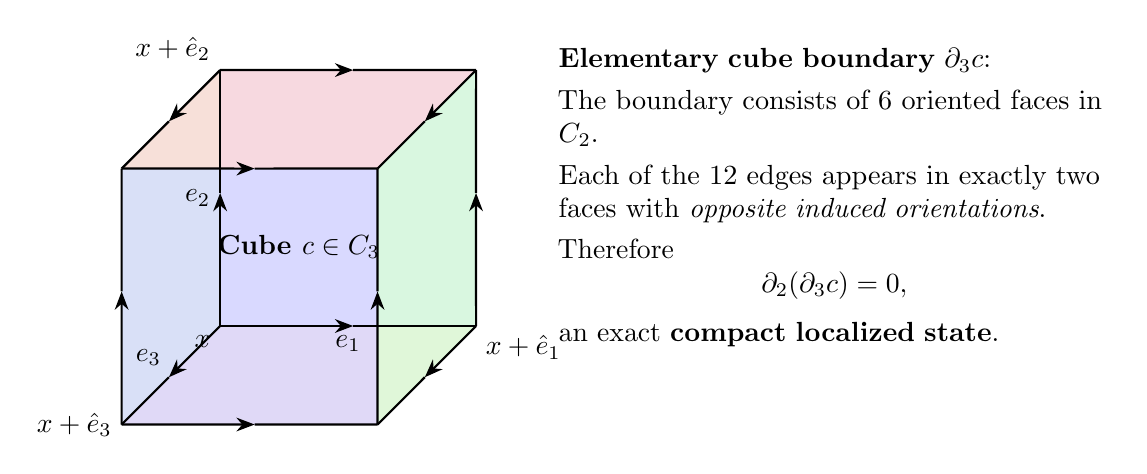
\begin{tikzpicture}[scale=1.3, >=Stealth]
  \coordinate (O) at (0,0,0);
  \coordinate (X) at (2.5,0,0);
  \coordinate (Y) at (0,2.5,0);
  \coordinate (Z) at (0,0,2.5);
  \coordinate (XY) at (2.5,2.5,0);
  \coordinate (XZ) at (2.5,0,2.5);
  \coordinate (YZ) at (0,2.5,2.5);
  \coordinate (XYZ) at (2.5,2.5,2.5);

  \fill[blue!10, opacity=0.7] (O) -- (X) -- (XY) -- (Y) -- cycle;
  \fill[green!10, opacity=0.7] (O) -- (Y) -- (YZ) -- (Z) -- cycle;
  \fill[red!10, opacity=0.7] (O) -- (Z) -- (XZ) -- (X) -- cycle;
  \fill[red!20, opacity=0.6] (Y) -- (XY) -- (XYZ) -- (YZ) -- cycle;
  \fill[green!20, opacity=0.6] (X) -- (XY) -- (XYZ) -- (XZ) -- cycle;
  \fill[blue!20, opacity=0.6] (Z) -- (XZ) -- (XYZ) -- (YZ) -- cycle;

  \draw[thick, ->] (O) -- (1.3,0,0); \draw[thick] (1.3,0,0) -- (X);
  \draw[thick, ->] (O) -- (0,1.3,0); \draw[thick] (0,1.3,0) -- (Y);
  \draw[thick, ->] (O) -- (0,0,1.3); \draw[thick] (0,0,1.3) -- (Z);
  \draw[thick, ->] (X) -- (2.5,1.3,0); \draw[thick] (2.5,1.3,0) -- (XY);
  \draw[thick, ->] (Y) -- (1.3,2.5,0); \draw[thick] (1.3,2.5,0) -- (XY);
  \draw[thick, ->] (X) -- (2.5,0,1.3); \draw[thick] (2.5,0,1.3) -- (XZ);
  \draw[thick, ->] (Z) -- (1.3,0,2.5); \draw[thick] (1.3,0,2.5) -- (XZ);
  \draw[thick, ->] (Y) -- (0,2.5,1.3); \draw[thick] (0,2.5,1.3) -- (YZ);
  \draw[thick, ->] (Z) -- (0,1.3,2.5); \draw[thick] (0,1.3,2.5) -- (YZ);
  \draw[thick, ->] (XY) -- (2.5,2.5,1.3); \draw[thick] (2.5,2.5,1.3) -- (XYZ);
  \draw[thick, ->] (XZ) -- (2.5,1.3,2.5); \draw[thick] (2.5,1.3,2.5) -- (XYZ);
  \draw[thick, ->] (YZ) -- (1.3,2.5,2.5); \draw[thick] (1.3,2.5,2.5) -- (XYZ);

  \node[below left] at (O) {$x$};
  \node[below right] at (X) {$x+\hat e_1$};
  \node[above left] at (Y) {$x+\hat e_2$};
  \node[left] at (Z) {$x+\hat e_3$};
  \node at (1.25, 1.25, 1.25) {\textbf{Cube $c \in C_3$}};
  \node[below] at (1.25,0,0) {$e_1$};
  \node[left] at (0,1.25,0) {$e_2$};
  \node[above left] at (0,0,1.25) {$e_3$};

  \node[text width=7cm, align=left] at (6, 1.25) {
    \textbf{Elementary cube boundary $\partial_3 c$}:\\[0.3em]
    The boundary consists of 6 oriented faces in $C_2$.\\[0.3em]
    Each of the 12 edges appears in exactly two faces with \emph{opposite induced orientations}.\\[0.3em]
    Therefore
    $$\partial_2 (\partial_3 c) = 0,$$
    an exact \textbf{compact localized state}.
  };
\end{tikzpicture}
\caption{The elementary $3$-cube boundary $\partial_3 c \in C_2$ forming a compact localized state. Every link is cancelled pairwise by adjacent faces carrying opposite orientations.}\label{fig:cls_cube}
\end{figure}

\subsection{Down-Laplacian and the Bloch Coboundary}

Equipping each $C_k$ with the inner product making the cell basis orthonormal, the adjoints $\partial_k\dg$ are the coboundaries, and the combinatorial Laplacians on $C_2$ are
\begin{equation}\label{eq:laplacians_def}
  \Ldn = \partial_2\dg\partial_2, \qquad \Lup = \partial_3\partial_3\dg, \qquad \Delta_2 = \Ldn + \Lup .
\end{equation}
The chain complex property gives the fundamental orthogonality
\begin{equation}\label{eq:Ldn_Lup_ortho}
  \Ldn\Lup = \partial_2\dg(\partial_2\partial_3)\partial_3\dg = 0, \qquad \Lup\Ldn = 0 .
\end{equation}

Passing to the Bloch basis by discrete Fourier transform on $\Lambda$, the $3$-cells, $2$-cells and $1$-cells give $1$, $3$ and $3$ orbitals per momentum $k \in (-\pi,\pi]^3$. Ordering the face orbitals as $p_1 = (1,2)$, $p_2 = (1,3)$, $p_3 = (2,3)$ and the link orbitals as $e_1,e_2,e_3$, and writing $d_j = e^{ik_j}-1$, the face-to-link coboundary is
\begin{equation}\label{eq:B_matrix}
  \Bc(k) = \begin{pmatrix} d_2 & -d_1 & 0 \\ d_3 & 0 & -d_1 \\ 0 & d_3 & -d_2 \end{pmatrix},
  \qquad
  \partial_2(k) = \Bc(k)\dg = \begin{pmatrix} \bar d_2 & \bar d_3 & 0 \\ -\bar d_1 & 0 & \bar d_3 \\ 0 & -\bar d_1 & -\bar d_2 \end{pmatrix}.
\end{equation}

\subsection{Proof of the Factorization Theorem}

\begin{theorem}[Down-Laplacian Factorization]\label{thm:factorization_proof}
Let $w(k) = (\bar d_3, -\bar d_2, \bar d_1)^T \in \C^3$ and
\begin{equation}\label{eq:qk_def}
  q(k) = \sum_{j=1}^3 |d_j|^2 = 4\sum_{j=1}^3 \sin^2\!\left(\frac{k_j}{2}\right).
\end{equation}
Then
\begin{equation}\label{eq:Ldn_proj}
  \Ldn(k) = \Bc(k)\Bc(k)\dg = q(k)I_3 - w(k)w(k)\dg,
\end{equation}
so that
\begin{equation}\label{eq:Ldn_spec}
  \spec(\Ldn(k)) = \{0, q(k), q(k)\},
\end{equation}
the zero mode being spanned by $\psi(k) = w(k)$ whenever $q(k) > 0$. Moreover $\Bc(k)\dg w(k) = 0$ identically in $k$.
\end{theorem}

\begin{proof}
Direct multiplication gives the diagonal entries
\begin{align*}
  (\Bc\Bc\dg)_{11} &= |d_2|^2 + |d_1|^2 = q - |d_3|^2 = q - |w_1|^2, \\
  (\Bc\Bc\dg)_{22} &= |d_3|^2 + |d_1|^2 = q - |d_2|^2 = q - |w_2|^2, \\
  (\Bc\Bc\dg)_{33} &= |d_3|^2 + |d_2|^2 = q - |d_1|^2 = q - |w_3|^2,
\end{align*}
and the off-diagonal entries
\begin{align*}
  (\Bc\Bc\dg)_{12} &= d_2\bar d_3 = -w_1\bar w_2, \qquad
  (\Bc\Bc\dg)_{13}  = -d_1\bar d_3 = -w_1\bar w_3, \\
  (\Bc\Bc\dg)_{23} &= d_1\bar d_2 = -w_2\bar w_3 .
\end{align*}
Since $\Bc\Bc\dg$ is Hermitian, every entry satisfies $(\Bc\Bc\dg)_{ij} = q\delta_{ij} - w_i\bar w_j$, which is \eqref{eq:Ldn_proj}. Next,
\begin{equation*}
  \Bc(k)\dg w(k) =
  \begin{pmatrix} \bar d_2 & \bar d_3 & 0 \\ -\bar d_1 & 0 & \bar d_3 \\ 0 & -\bar d_1 & -\bar d_2 \end{pmatrix}
  \begin{pmatrix} \bar d_3 \\ -\bar d_2 \\ \bar d_1 \end{pmatrix}
  = \begin{pmatrix} \bar d_2\bar d_3 - \bar d_3\bar d_2 \\ -\bar d_1\bar d_3 + \bar d_3\bar d_1 \\ \bar d_1\bar d_2 - \bar d_2\bar d_1\end{pmatrix} = 0,
\end{equation*}
whence $\Ldn w = \Bc(\Bc\dg w) = 0$. For $v \perp w$ we get $\Ldn v = (qI_3 - ww\dg)v = qv$, and $w^\perp$ is two-dimensional when $q(k)>0$, so the eigenvalue $q(k)$ has multiplicity two.
\end{proof}

\begin{figure}[htbp]
\centering
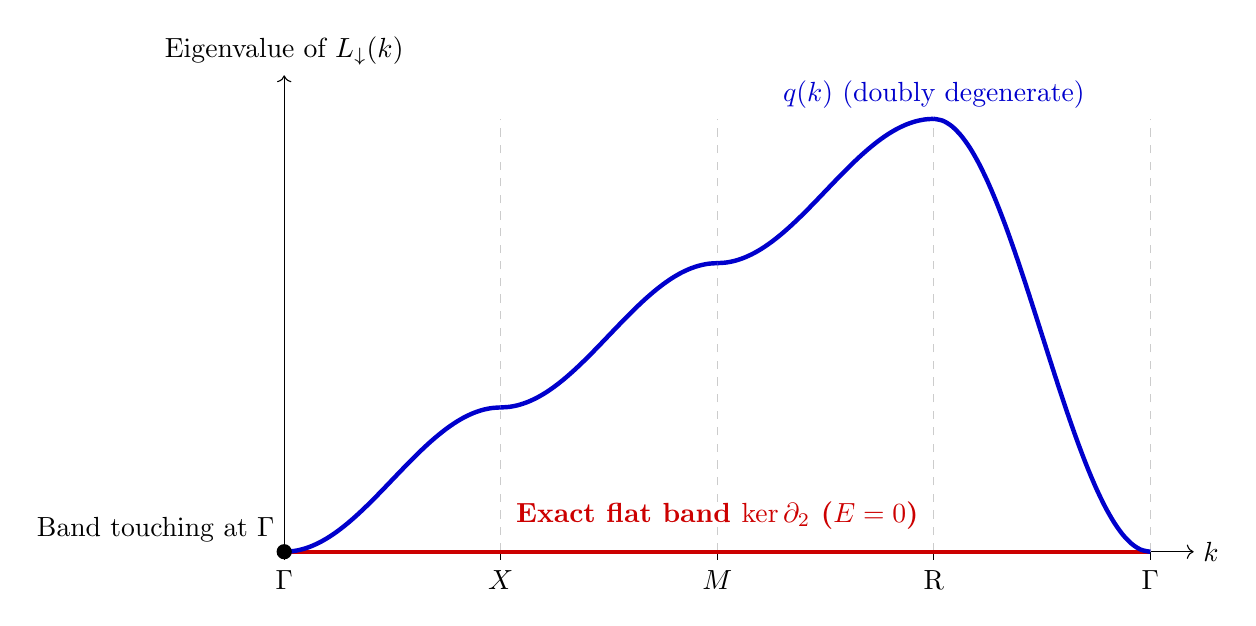
\begin{tikzpicture}[scale=1.1]
  \draw[->] (0,0) -- (10.5,0) node[right] {$k$};
  \draw[->] (0,0) -- (0,5.5) node[above] {Eigenvalue of $\Ldn(k)$};

  \draw (0,0.1) -- (0,-0.1) node[below] {$\Gamma$};
  \draw (2.5,0.1) -- (2.5,-0.1) node[below] {$X$};
  \draw (5.0,0.1) -- (5.0,-0.1) node[below] {$M$};
  \draw (7.5,0.1) -- (7.5,-0.1) node[below] {$\mathrm{R}$};
  \draw (10.0,0.1) -- (10.0,-0.1) node[below] {$\Gamma$};

  \draw[dashed, gray!40] (2.5,0) -- (2.5,5);
  \draw[dashed, gray!40] (5.0,0) -- (5.0,5);
  \draw[dashed, gray!40] (7.5,0) -- (7.5,5);
  \draw[dashed, gray!40] (10.0,0) -- (10.0,5);

  \draw[ultra thick, red!80!black] (0,0) -- (10,0);
  \node[above, red!80!black] at (5, 0.15) {\textbf{Exact flat band $\ker \partial_2$ ($E = 0$)}};

  \draw[domain=0:2.5, smooth, variable=\x, blue!80!black, ultra thick]
    plot ({\x}, {1.666 * 4 * (sin(\x/2.5 * 90))^2 / 4});
  \draw[domain=2.5:5.0, smooth, variable=\x, blue!80!black, ultra thick]
    plot ({\x}, {1.666 * (4 + 4 * (sin((\x-2.5)/2.5 * 90))^2) / 4});
  \draw[domain=5.0:7.5, smooth, variable=\x, blue!80!black, ultra thick]
    plot ({\x}, {1.666 * (8 + 4 * (sin((\x-5.0)/2.5 * 90))^2) / 4});
  \draw[domain=7.5:10.0, smooth, variable=\x, blue!80!black, ultra thick]
    plot ({\x}, {1.666 * 12 * (cos((\x-7.5)/2.5 * 90))^2 / 4});

  \node[above, blue!80!black] at (7.5, 5.0) {$q(k)$ (doubly degenerate)};
  \fill[black] (0,0) circle (2.5pt);
  \node[above left] at (0,0) {Band touching at $\Gamma$};
\end{tikzpicture}
\caption{Universal second-order spectrum of $\Ldn = \Bc\Bc\dg$ along $\Gamma$--$X$--$M$--$\mathrm{R}$--$\Gamma$. The homological flat band at eigenvalue $0$ is protected by $\partial_2$ and touches the doubly degenerate branch $q(k)$ at $\Gamma$.}\label{fig:flat_band_dispersion}
\end{figure}

\section{Topological Zero-Mode Multiplicity and Compact Localized States}\label{sec:multiplicity}

\subsection{Exact Real-Space Multiplicity}

\begin{theorem}[Torus Carrier Multiplicity]\label{thm:carrier_multiplicity}
For $\Lambda = (\Z/L\Z)^3$ with $L \ge 3$,
\begin{equation}\label{eq:dim_ker_d2}
  \dim\ker\partial_2 = (L^3-1) + 3 = L^3 + 2 .
\end{equation}
\end{theorem}

\begin{proof}
By discrete Hodge theory on finite cell complexes \cite{Eckmann1944,Forman1998} the $2$-cycles decompose orthogonally as
\begin{equation}\label{eq:hodge_cycle_decomp}
  \ker\partial_2 = \operatorname{im}\partial_3 \oplus \mathcal{H}_2(T^3), \qquad \mathcal{H}_2(T^3) \cong H_2(T^3;\R).
\end{equation}
For the boundaries, $\dim C_3 = L^3$ and there are no $4$-cells, so $b_3(T^3) = \dim\ker\partial_3 = 1$ and rank-nullity gives
\begin{equation}
  \dim\operatorname{im}\partial_3 = L^3 - b_3(T^3) = L^3 - 1 .
\end{equation}
The single relation among the $L^3$ cube boundaries is the global sum
\begin{equation}\label{eq:cube_sum_relation}
  \sum_{x\in\Lambda}\partial_3[x;1,2,3] = 0,
\end{equation}
since on the periodic torus each oriented face lies in exactly two cubes with opposite induced orientation. For the harmonic part, $\dim\mathcal{H}_2(T^3) = b_2(T^3) = \binom{3}{2} = 3$, represented by the non-contractible wrapping sheets
\begin{equation}\label{eq:toron_sheets}
  S_\mu = \sum_{x\in\Lambda,\ x_\mu = 0}[x;(\mu)^c], \qquad \mu\in\{1,2,3\},
\end{equation}
each closed ($\partial_2 S_\mu = 0$) but not a boundary, since it wraps the torus. Adding the two orthogonal contributions gives \eqref{eq:dim_ker_d2}.
\end{proof}

\subsection{Compact Localized States and the Singular Band Crossing}

Each cube boundary $c_x = \partial_3[x;1,2,3]$ is supported on exactly six plaquettes and satisfies $\partial_2 c_x = 0$, hence has zero hopping amplitude to anything outside its support: the $L^3-1$ independent boundaries form a macroscopic family of compact localized states. They do not, however, span the carrier, and the obstruction is topological.

\begin{proposition}[Singular Band Crossing]\label{prop:singular_crossing}
The normalized Bloch carrier
\begin{equation}
  \hat\psi(k) = \frac{w(k)}{\sqrt{q(k)}}
  = \frac{1}{\sqrt{\sum_j|e^{ik_j}-1|^2}}\begin{pmatrix} e^{-ik_3}-1 \\ -(e^{-ik_2}-1) \\ e^{-ik_1}-1\end{pmatrix}
\end{equation}
has no continuous limit as $k \to 0$: along the ray $k = t\hat n$ with $t>0$ and $\hat n = (n_1,n_2,n_3)$ a unit vector,
\begin{equation}
  \lim_{t\to 0^+}\hat\psi(t\hat n) = -i\begin{pmatrix} n_3 \\ -n_2 \\ n_1\end{pmatrix},
\end{equation}
which depends on $\hat n$.
\end{proposition}

Because $\hat\psi$ is non-analytic at $\Gamma$, the band is a \emph{singular} flat band in the classification of Rhim and Yang \cite{Rhim2019,BergmanWuBalents2008}. This is exactly why purely local compact states cannot form a complete Wannier basis for the carrier: the three global toron sheets $S_1,S_2,S_3$ are required, and the counting $L^3 = (L^3-1)+1$ of cube boundaries plus their one relation falls three short of $\dim\ker\partial_2$ without them.

\begin{remark}[The band is singular at $\Gamma$ but the energy is not]\label{rem:gamma_reconciliation}
Proposition~\ref{prop:singular_crossing} and Theorem~\ref{thm:intro_dispersion} are compatible, and the distinction matters. The carrier \emph{eigenvector} $\hat\psi(k)$ has no limit at $\Gamma$. The carrier \emph{energy} does: the fourth-order invariant $D_N(k)$ of \eqref{eq:intro_DN} is a polynomial in the $X_i$ with $D_N(\Gamma) = 0$, and the normalized branch value $D_N(k)/q(k)$ vanishes as $k\to 0$ along every ray, since $D_N = O(|k|^4)$ while $q = O(|k|^2)$. So the band energy extends continuously by $0$ at $\Gamma$ even though no continuous choice of carrier eigenvector exists there. Statements below that call $\Gamma$ the band minimum refer to this continuous extension of the energy, not to a choice of eigenvector.
\end{remark}

\section{Universal All-Rank Hopping Coefficient \texorpdfstring{$t_N \in \Q(N)$}{t\_N in Q(N)}}\label{sec:weingarten}

\subsection{Weingarten Integration across Fusion Channels}

At second order in degenerate perturbation theory the effective Hamiltonian on the one-plaquette manifold is
\begin{equation}\label{eq:H2_resolvent}
  H_2 = -\,P_- V \frac{Q}{H_E - 2\CF} V P_-,
\end{equation}
with $P_-$ the projector onto $\mathcal{H}^{(1)}_-$ and $Q = 1 - P_-$. Two distinct plaquettes $p, p'$ can interact through $V$ only if they share at least one link: otherwise the Haar integral over an unshared link vanishes, $\int_{\SU(N)}U_{ij}\,dU = 0$. For nearest-neighbour plaquettes sharing exactly one link $\ell$, six unshared fundamental links remain excited in the intermediate state.

On the shared link the fusion depends on the relative induced orientation:
\begin{equation}
  \text{opposite orientation:}\quad F\otimes\bar F = \mathbf{1}\oplus\Adj,
  \qquad
  \text{same orientation:}\quad F\otimes F = \Lambda^2 F\oplus\Sym^2 F .
\end{equation}

\subsection{Exact Evaluation of Channel Resolvent Weights}

Let $\rho\in\{\mathbf{1},\Adj,\Lambda^2F,\Sym^2F\}$. The six unshared links contribute $6\cdot\tfrac12\CF = 3\CF$ and the shared link contributes $\tfrac12 C_2(\rho)$, so the energy denominator in \eqref{eq:H2_resolvent} is
\begin{equation}\label{eq:Delta_E_rho}
  \Delta E_\rho = \left(3\CF + \tfrac{1}{2}C_2(\rho)\right) - 2\CF = \CF + \tfrac{1}{2}C_2(\rho).
\end{equation}
By Weingarten calculus on $\SU(N)$ \cite{Weingarten1978,CollinsSniady2006} the projection of the shared-link tensor product onto $\rho$ carries squared norm $d_\rho/N^2$ with $d_\rho = \dim\rho$, so the resolvent weight is
\begin{equation}\label{eq:w_rho}
  w_\rho = -\,\frac{d_\rho/N^2}{\CF + \tfrac12 C_2(\rho)} .
\end{equation}
Table~\ref{tab:channels} records the four evaluations; each entry is \eqref{eq:w_rho} with the stated $d_\rho$ and $C_2(\rho)$, and the identity has been checked symbolically over $\Q(N)$.

\begin{table}[htbp]
\centering
\caption{Dimensions, quadratic Casimirs and resolvent weights for the four shared-link fusion channels in $\SU(N)$.}\label{tab:channels}
\vspace{0.5em}
\begin{tabular}{@{}lccc@{}}
\toprule
Channel $\rho$ & Dimension $d_\rho$ & Casimir $C_2(\rho)$ & Resolvent weight $w_\rho$ \\
\midrule
Singlet $\mathbf{1}$ & $1$ & $0$ & $-\dfrac{2}{N(N-1)(N+1)}$ \\[1em]
Adjoint $\Adj$ & $N^2-1$ & $N$ & $-\dfrac{2(N-1)(N+1)}{N(2N^2-1)}$ \\[1em]
Antisymmetric $\Lambda^2 F$ & $\dfrac{N(N-1)}{2}$ & $\dfrac{(N+1)(N-2)}{N}$ & $-\dfrac{N-1}{(N+1)(2N-3)}$ \\[1em]
Symmetric $\Sym^2 F$ & $\dfrac{N(N+1)}{2}$ & $\dfrac{(N-1)(N+2)}{N}$ & $-\dfrac{N+1}{(N-1)(2N+3)}$ \\
\bottomrule
\end{tabular}
\end{table}

\subsection{Proof of the All-Rank Hopping Formula}

\begin{theorem}[All-Rank Shared-Link Theorem]\label{thm:tN_derivation}
For every integer $N \ge 3$,
\begin{equation}\label{eq:tN_closed}
  t_N = \frac{2N(N^2-4)}{(N^2-1)(2N^2-1)(4N^2-9)} \in \Q(N).
\end{equation}
\end{theorem}

\begin{proof}
Summing the opposite-orientation channels,
\begin{equation}\label{eq:Wopp_sum}
  \Wopp = w_{\mathbf{1}} + w_{\Adj} = -\frac{2}{N(N^2-1)} - \frac{2(N^2-1)}{N(2N^2-1)} = -\frac{2N^3}{(N^2-1)(2N^2-1)},
\end{equation}
and the same-orientation channels,
\begin{align}\label{eq:Wsame_sum}
  \Wsame &= w_{\Lambda^2} + w_{\Sym^2} = -\frac{N-1}{(N+1)(2N-3)} - \frac{N+1}{(N-1)(2N+3)} \notag \\
    &= -\frac{(N-1)^2(2N+3) + (N+1)^2(2N-3)}{(N^2-1)(4N^2-9)} = -\frac{4N(N^2-2)}{(N^2-1)(4N^2-9)} .
\end{align}
In the charge-odd combination $|p,-\rangle$ the two orientation classes enter with opposite sign, so the signed shared-link adjacency $\Ssq = \Ldn - 4I$ is multiplied by the net difference $t_N = \Wsame - \Wopp$:
\begin{align*}
  t_N &= -\frac{4N(N^2-2)}{(N^2-1)(4N^2-9)} + \frac{2N^3}{(N^2-1)(2N^2-1)}
      = \frac{2N}{N^2-1}\left[\frac{N^2}{2N^2-1} - \frac{2(N^2-2)}{4N^2-9}\right] \\
      &= \frac{2N}{N^2-1}\left[\frac{N^2(4N^2-9) - 2(N^2-2)(2N^2-1)}{(2N^2-1)(4N^2-9)}\right] \\
      &= \frac{2N}{N^2-1}\left[\frac{4N^4-9N^2 - (4N^4-10N^2+4)}{(2N^2-1)(4N^2-9)}\right]
      = \frac{2N(N^2-4)}{(N^2-1)(2N^2-1)(4N^2-9)} .
\end{align*}
Absorbing the resulting $-4t_N I$ into the diagonal scalar energy gives $H_2 = E_{\mathrm{flat},N}I + t_N\Ldn$.
\end{proof}

\begin{corollary}[Properties of $t_N$]\label{cor:tN_properties}
\begin{enumerate}\itemsep1pt
  \item \textbf{$\SU(2)$ vanishing.} $t_2 = 0$. This reflects pseudo-reality: for $\SU(2)$ charge conjugation is inner, $U^* = \sigma_2 U\sigma_2$, so $\Tr U_p = \Tr U_p\dg$ and the charge-odd state \eqref{eq:plaquette_basis} is identically zero. The vanishing of $t_N$ at $N=2$ is thus not an accident of the algebra but the statement that the sector itself is empty.
  \item \textbf{$\SU(3)$ match.} $t_3 = \dfrac{2\cdot3\cdot5}{8\cdot17\cdot27} = \dfrac{30}{3672} = \dfrac{5}{612}$, agreeing with the series of Hamer \cite{Hamer1989} to all printed digits.
  \item \textbf{Strict positivity.} For $N\ge3$ each of $N^2-4$, $N^2-1$, $2N^2-1$, $4N^2-9$ is positive, so $t_N>0$.
  \item \textbf{Large-$N$ asymptotics.}
  $t_N = \dfrac{1}{4N^3} - \dfrac{1}{16N^5} - \dfrac{77}{64N^7} - \dfrac{1021}{256N^9} + O(N^{-11})$.
\end{enumerate}
\end{corollary}

\section{Single-Face Free-Fermion Theorem and All-Order Channel Cancellation}\label{sec:fermion}

\subsection{Mapping the \texorpdfstring{$\U(N)$}{U(N)} Plaquette to \texorpdfstring{$N$}{N} Fermions in a Mathieu Well}

Let $U\in\U(N)$ be the holonomy around a single face. A gauge-invariant wavefunction $\Psi(U)$ is a class function of the eigenvalues $e^{i\theta_1},\dots,e^{i\theta_N}$. By Weyl integration,
\begin{equation}
  dU = \frac{1}{N!}\prod_{j=1}^N\frac{d\theta_j}{2\pi}\,|\Delta(e^{i\theta})|^2,
  \qquad \Delta(e^{i\theta}) = \prod_{1\le j<k\le N}(e^{i\theta_j} - e^{i\theta_k}),
\end{equation}
so multiplication by the Vandermonde determinant carries symmetric functions to totally antisymmetric wavefunctions of $N$ spinless fermions on a circle. Characters $\chi_\lambda(U)$ become Slater determinants $|p_1,\dots,p_N\rangle$ with
\begin{equation}
  p_j = \lambda_j - j + \tfrac{N+1}{2} \in
  \begin{cases}\Z, & N \text{ odd},\\[2pt] \Z + \tfrac12, & N \text{ even},\end{cases}
  \qquad P = \sum_j p_j = |\lambda| \ \ (\text{the } N\text{-ality}),
\end{equation}
the singlet being the filled Fermi sea $\{-\tfrac{N-1}{2},\dots,\tfrac{N-1}{2}\}$.

\begin{theorem}[Single-Face Free-Fermion Representation]\label{thm:free_fermion}
In the Slater determinant basis,
\begin{equation}\label{eq:H_SU_fermion}
  H_{\SU(N)} = H_{\U(N)} - \frac{P^2}{N},
  \qquad
  H_{\U(N)} = \sum_{j=1}^N\left[p_j^2 + u\left(e^{i\theta_j} + e^{-i\theta_j}\right)\right] = \sum_{j=1}^N\left[p_j^2 + 2u\cos\theta_j\right].
\end{equation}
\end{theorem}

\begin{proof}
By the Freudenthal--de~Vries strange formula applied to $\SU(N)$, for a highest weight $\lambda_1\ge\cdots\ge\lambda_N = 0$,
\begin{equation*}
  2C_2(\lambda) = \sum_{j=1}^N p_j^2 - \frac{P^2}{N} - E_{\mathrm{sea}},
  \qquad E_{\mathrm{sea}} = \sum_{j=1}^N\left(-j + \tfrac{N+1}{2}\right)^2 = \frac{N(N^2-1)}{12} .
\end{equation*}
(This identity has been verified in exact rational arithmetic for all four channels of Table~\ref{tab:channels} and all $3\le N\le14$.) The magnetic perturbation $V = \Tr U + \Tr U\dg = \sum_j(e^{i\theta_j} + e^{-i\theta_j})$ shifts the momentum of exactly one fermion by $\pm1$,
\begin{equation*}
  e^{i\theta}|p\rangle = |p+1\rangle, \qquad e^{-i\theta}|p\rangle = |p-1\rangle,
\end{equation*}
so $V$ is a one-body operator and $H_{\U(N)}$ separates into $N$ uncoupled copies of the Mathieu operator $h = p^2 + 2u\cos\theta$.
\end{proof}

\subsection{The \texorpdfstring{$\U(N)$}{U(N)} Doublet Does Not Split}

The physical object is the charge-parity splitting of the one-plaquette doublet,
\begin{equation}\label{eq:Sm_def}
  S_m = \mathrm{odd}_m - \mathrm{even}_m = -2\,K_m[F][\bar F],
\end{equation}
where $K_m$ is the order-$m$ coefficient of the Bloch effective Hamiltonian on the model space $\{\chi_F,\chi_{\bar F}\}$. In the fermion language the doublet is
\begin{equation}
  F = \text{sea with } \tfrac{N-1}{2}\to\tfrac{N+1}{2} \ (P = +1),
  \qquad
  \bar F = \text{sea with } -\tfrac{N-1}{2}\to-\tfrac{N+1}{2} \ (P = -1),
\end{equation}
both at unperturbed energy $N - 1/N$.

\begin{theorem}[$\U(N)$ Doublet Non-Splitting]\label{thm:doublet_non_splitting}
In the $\U(N)$ model of \eqref{eq:H_SU_fermion}, i.e. with the centre-of-mass term deleted, the Bloch effective Hamiltonian on $\{F,\bar F\}$ satisfies
\begin{equation}\label{eq:Km_zero}
  K_m[F][\bar F] = 0 \qquad \text{for every } m \le N-2 .
\end{equation}
Equivalently $\mathrm{odd}_m = \mathrm{even}_m$ in that model, at every order and rank in this range.
\end{theorem}

\begin{proof}
$H_{\U(N)}$ is a sum of one-body operators $h = p^2 + u(T + T\dg)$ on $\ell^2$ of the momentum lattice. Hence its exact eigenstates are Slater determinants of exact eigenvectors of $h$, and its exact eigenvalues are sums of one-particle eigenvalues.

The one-particle levels $p^2$ are degenerate in pairs $\{+p,-p\}$. Since $T + T\dg$ shifts $p$ by one, the two members of a pair are connected only by a walk of length $2|p|$, so their splitting is $O(u^{2|p|})$: this is the Mathieu band-gap law \cite{McLachlan1947,AbramowitzStegun1964}.

Write $A = \{\pm\tfrac{N-1}{2}\}$ for the Fermi pair and $B = \{\pm\tfrac{N+1}{2}\}$ for the first empty pair. Both $F$ and $\bar F$ fill every pair with $|p|\le\tfrac{N-3}{2}$ completely and occupy exactly one member of $A$ and one member of $B$. The same is true of the two remaining states of this unperturbed multiplet,
\begin{equation*}
  D_\pm \;=\; \text{inner sea} \;\cup\; \left\{\pm\tfrac{N-1}{2}, \pm\tfrac{N+1}{2}\right\},
\end{equation*}
which are $\det U$ and $\det U^{-1}$ times the sea, of momentum $\pm N$. Reaching $D_\pm$ from the doublet requires at least $N-1$ elementary hops, so $D_\pm$ is absent from every $K_m$ with $m\le N-2$ and the model space $\{F,\bar F\}$ is well defined in that range.

The four exact eigenvalues in this sector are $e_A^{\pm} + e_B^{\pm}$ plus the common inert-sea energy, with
\begin{equation}\label{eq:mathieu_gaps}
  \delta_A := e_A^+ - e_A^- = O(u^{N-1}), \qquad \delta_B := e_B^+ - e_B^- = O(u^{N+1}).
\end{equation}
The Bloch operator $K(u)$ on the two-dimensional model space is a formal power series in $u$ whose eigenvalues are the exact eigenvalues of the two perturbed states reducing to $F$ and $\bar F$, and whose eigenvectors are their projections onto the model space; these projections are linearly independent at $u=0$ and hence as formal series. A diagonalisable $K = S\,\diag(E, E+\delta)\,S^{-1}$ with $\delta = O(u^{N-1})$ equals $E\,I + O(u^{N-1})$, so $K_m[F][\bar F] = 0$ for $m \le N-2$.
\end{proof}

\begin{remark}[A natural but incorrect argument]\label{rem:pauli_fallacy}
It is tempting to argue instead that $F$ and $\bar F$ cannot be connected below order $N-1$ because a fermion would have to traverse the whole Fermi sea, a momentum change of $\Delta p = N+1$, and $V$ moves momentum by one unit per insertion. \emph{This argument is false.} The perturbation is a sum of one-body operators, so distinct insertions may move \emph{distinct} fermions; $F$ and $\bar F$ differ by moving one fermion down by one unit and another up by one unit, which is reachable in two hops. For $N=3$, for instance, $F = \{-1,0,2\}$ and $\bar F = \{-2,0,1\}$ are joined at second order through both $\{-2,0,2\}$ and $\{-1,0,1\}$. Those two second-order paths are individually non-zero; they cancel because their energy denominators are $+\Delta$ and $-\Delta$. The correct mechanism is not Pauli blocking of a single crossing but the additive structure of the free-fermion spectrum together with the Mathieu band-gap law, as in the proof above.
\end{remark}

\begin{observation}[The vanishing range is wider than Theorem~\ref{thm:doublet_non_splitting} proves]\label{obs:2N}
Theorem~\ref{thm:doublet_non_splitting} is limited by the states $D_\pm$, which make the two-dimensional model space singular beyond order $N-2$. On the \emph{four}-dimensional multiplet $\{F,\bar F,D_+,D_-\}$, which is the full unperturbed degenerate space and is well defined at every order, the Bloch operator $K = W\diag(E)W^{-1}$ can be computed directly from the one-body spectrum. Doing so in $60$-digit arithmetic for $N = 3,4,5,6$ gives
\begin{equation}\label{eq:2N_law}
  K[F][\bar F] \;=\; \frac{N-2}{4}\,\delta_A\,\delta_B\,\bigl(1 + O(u^2)\bigr),
\end{equation}
with fitted powers $2N = 6,8,10,12$ and ratios $K/(\delta_A\delta_B) = 0.250, 0.500, 0.750, 1.000$ reproducing $(N-2)/4$ to six digits. Since $\delta_A = O(u^{N-1})$ and $\delta_B = O(u^{N+1})$, this says $K_m[F][\bar F] = 0$ for all $m \le 2N-1$.

The leading-order mechanism is transparent. On the multiplet the additivity of the spectrum gives
$K = \bar E\,I + \tfrac{\delta_A}{2}\,W Z_A W^{-1} + \tfrac{\delta_B}{2}\,W Z_B W^{-1}$,
where $Z_A, Z_B$ are the two commuting pair-label signs. If $W$ were exactly the parity transform, both conjugates would be single-label flips, and since $F$ and $\bar F$ differ in \emph{both} labels the element would vanish identically: a sum of one-label operators cannot flip two labels at once. The residue \eqref{eq:2N_law} comes only from the cross terms in $W$.

Bounding those cross terms is not carried out here. It has since been carried out in the companion manuscript \cite{Companion2026}, whose Theorem~6.2 evaluates the Bloch element in closed form,
\begin{equation}\label{eq:exactK}
  \langle F|K^{\mathrm{B}}|\bar F\rangle
  = \frac{\delta_A - \delta_B}{4}\cdot\frac{r_1 - r_2}{1 - r_1r_2},
  \qquad r_1 = \frac{x^+}{Y^-},\quad r_2 = \frac{x^-}{Y^+},
\end{equation}
by expanding the overlap determinant along the inert inner block: the $2\times2$ minors are generalised Vandermonde determinants of a half-line Jacobi matrix, and a trace identity gives $r_1 - r_2 = (N-2)\delta_B(1+O(u))$, which is \eqref{eq:2N_law}. That argument confirms the mechanism stated above --- if the overlaps factorised over the two labels the element would vanish identically, and it is exactly the exchange term of the minor that survives --- and upgrades \eqref{eq:2N_law} to a theorem for the Bloch (non-Hermitian) effective Hamiltonian. The corresponding statement for the Hermitian des~Cloizeaux form is not covered by either treatment.

Nothing in the present paper depends on \eqref{eq:2N_law}: Theorem~\ref{thm:doublet_non_splitting}, with its range $m\le N-2$, is what the results below use.
\end{observation}

\subsection{Consequences, and the Status of the Grading Law}\label{sec:fermion_status}

\begin{corollary}[All-Order Channel Cancellation]\label{cor:channel_cancel}
Decomposing $S_m$ by intermediate irrep decomposes the same set of paths in the $\U(N)$ and $\SU(N)$ models. The $\SU(N)$ energies differ from the $\U(N)$ ones only by $-(P_i^2-1)/N$ on each intermediate state, a relative $O(N^{-2})$ correction to denominators of size $\sim N$. Hence for fixed $m$ and $N$ large enough that $m\le N-2$, every channel's leading $N^{-(m-1)}$ coefficient equals its $\U(N)$ value. Since those sum to zero by Theorem~\ref{thm:doublet_non_splitting}, the four channel weights
\begin{equation}\label{eq:channel_cancel}
  (\mathbf{1},\ \Adj,\ \Sym^2,\ \Lambda^2) \longmapsto (-4,\, +2,\, +1,\, +1)\,2^{m/2-2},
  \qquad -4+2+1+1 = 0,
\end{equation}
cancel at every even order $m$, and consequently
\begin{equation}\label{eq:grading_law}
  S_m = O\!\left(N^{-(m+1)}\right).
\end{equation}
\end{corollary}

\begin{remark}[Exact reduction and the open tower (T)]\label{rem:tower}
$S_m^{\SU(N)}$ is exactly the difference between the same Bloch sum evaluated with denominators $E_F - E_i - (P_i^2-1)/N$ and with $E_F - E_i$; that is, the splitting is generated entirely by the centre-of-mass term. Writing that term as $-\lambda P^2/N$, the quantity $S_m(\lambda)$ is a polynomial in $\lambda$ with zero constant term, and its coefficients for $1\le j\le m/2$ are each $O(N^{-(2m-1)})$ while those with $j>m/2$ fall faster. The remaining content of the sharper law is therefore the statement
\begin{quote}
  \textbf{(T)} \quad for $1\le j<m/2$, the $j$-fold insertion of $(P^2-1)/N$ into the $\U(N)$ Bloch sum, whose natural size is $N^{-(m-1)-2j}$, is in fact $O(N^{-(2m-1)})$.
\end{quote}
\emph{(T) is not proved here.} It is supported numerically at the orders computed. Consequently the law established in this paper is \eqref{eq:grading_law}, $S_m = O(N^{-(m+1)})$, and \emph{not} the stronger $S_m = O(N^{-(2m-1)})$ that appears in the source ledger. Any downstream use of the stronger exponent inherits (T) as a hypothesis.
\end{remark}

\section{Fourth-Order Hodge Decomposition and the Tier Collapse}\label{sec:hodge}

\subsection{The Plaquette Hodge Laplacian}

On the periodic cubical complex $C_2$ admits the discrete Hodge decomposition
\begin{equation}\label{eq:hodge_c2}
  C_2 = \operatorname{im}\partial_2\dg \oplus \ker\Delta_2 \oplus \operatorname{im}\partial_3 .
\end{equation}
In Bloch space each fiber $C_2(k)\cong\C^3$ satisfies a sharper identity.

\begin{proposition}[Fibre Laplacian Sum]\label{prop:fiber_laplacian_sum}
For every $k$,
\begin{equation}\label{eq:Ldn_plus_Lup}
  \Ldn(k) + \Lup(k) = q(k)\,I_3 .
\end{equation}
\end{proposition}

\begin{proof}
The map $\partial_3(k) : C_3(k)\to C_2(k)$ sends the single cube orbital to the column $w(k) = (\bar d_3,-\bar d_2,\bar d_1)^T$, so $\Lup(k) = \partial_3\partial_3\dg = w w\dg$. By Theorem~\ref{thm:factorization_proof}, $\Ldn = qI_3 - ww\dg$; adding gives \eqref{eq:Ldn_plus_Lup}.
\end{proof}

\subsection{The Feshbach Complement and \texorpdfstring{$\Rc$}{R}-Linearity}

\begin{proposition}[The Feshbach Projector]\label{prop:feshbach_proj}
At each $k$ with $q(k)>0$ the carrier is the line spanned by $\psi(k) = w(k)$, and the projector onto its orthogonal complement is
\begin{equation}\label{eq:feshbach_Q}
  Q(k) = I_3 - \frac{w w\dg}{q} = \frac{1}{q(k)}\Ldn(k),
\end{equation}
which is identically the projector onto $\ker\Lup(k)$. Consequently
\begin{equation}\label{eq:Q_annihilates_Hodge}
  Q\,\Ldn\,\psi = 0, \qquad Q\,\Lup\,\psi = 0 .
\end{equation}
\end{proposition}

\begin{proof}
$\Ldn\psi = 0$ gives $Q\Ldn\psi = 0$; and $\Lup\psi = q\psi$ with $Q\psi = 0$ gives $Q\Lup\psi = q\,Q\psi = 0$.
\end{proof}

Proposition~\ref{prop:feshbach_proj} has a decisive consequence: \emph{neither Hodge generator can induce a transition out of the carrier}. Any excursion into the virtual sector must therefore be mediated by an operator outside the Hodge algebra. Writing $\Ssq = \Ldn - 4I_3$ for the signed shared-link adjacency and splitting it into same-plane and cross-plane parts,
\begin{equation}
  \Ssq = S_\parallel + \Rc,
\end{equation}
we obtain the following.

\begin{corollary}[$\Rc$-Linearity]\label{cor:R_linearity}
Every excursion out of the carrier costs at least one insertion of $\Rc$, and the first excitation $\phi(k) = Q(k)\Rc(k)\psi(k)$ is strictly up-harmonic:
\begin{equation}
  \Lup(k)\bigl(Q(k)\Rc(k)\psi(k)\bigr) = 0 .
\end{equation}
\end{corollary}

\subsection{Fourth-Order Hodge Representation and Tier Collapse}

The $189$ independent matrix elements of the fourth-order kernel are spanned by the operator support
\begin{equation}\label{eq:support_set}
  \mathcal{S}_4 = \{\,I_3,\ \Ssq,\ \Ssq^2,\ \Lup,\ \Rc\,\}.
\end{equation}

\begin{theorem}[Fourth-Order Hodge Representation]\label{thm:hodge_decomp}
On all $189$ records of the fourth-order kernel,
\begin{equation}\label{eq:H4_hodge}
  H_4 = -\tilde\nu\,(\Lup - 2I) + \Utwo\,\Ssq^2 - \tilde\pi\,\Ssq + \tilde\sigma\,I - 2\,\Cshp\,\Rc,
  \qquad \tilde\nu = -\tfrac{5}{48},
\end{equation}
where $\Utwo$ is the two-hop cluster cumulant of Section~\ref{sec:dispersion} (not the coupling $u$ of \eqref{eq:u_def}).
\end{theorem}

Let $a_i = 4\sin^2(k_i/2)$, $q = a_1+a_2+a_3$, and let $e_2 = \sum_{i<j}a_ia_j$, $e_3 = a_1a_2a_3$ be the elementary symmetric polynomials. The projected carrier energy is $\varepsilon_4(k) = \langle\psi,H_4\psi\rangle/\langle\psi,\psi\rangle = \langle\psi,H_4\psi\rangle/q$. Clearing $q$, the general symmetry-allowed shape ansatz is
\begin{equation}\label{eq:shape_ansatz}
  q\,\varepsilon_4(k) = c_0\,q + \Ashp\,q^2 + 4\,\Cshp\,e_2 + \Bshp\,(q\,e_2) + \Dshp\,e_3 .
\end{equation}
The monomials $q e_2$ and $e_3$ are of degree three in the $a_i$ and scale as $|k|^6$ near $\Gamma$; they constitute the top tier of the ansatz.

\begin{theorem}[Hodge--Feshbach Tier Collapse]\label{thm:tier_collapse}
For the operator support $\mathcal{S}_4$, the carrier symbols $\sigma(W) = \langle\psi,W\psi\rangle$ are
\begin{equation}\label{eq:carrier_symbols}
  \sigma(I) = q, \quad \sigma(\Ssq) = -4q, \quad \sigma(\Ssq^2) = 16q, \quad \sigma(\Lup) = q^2, \quad \sigma(\Rc) = -2e_2 .
\end{equation}
Every symbol lies in $\operatorname{span}_\Q\{q,q^2,e_2\}$, so neither $qe_2$ nor $e_3$ receives any amplitude:
\begin{equation}\label{eq:B_D_zero}
  \Bshp = 0, \qquad \Dshp = 0 .
\end{equation}
\end{theorem}

\begin{proof}
The first four identities follow from $\Ldn\psi = 0$, $\Lup\psi = q\psi$ and $\Ssq\psi = -4\psi$. For the cross-plane operator, $\Rc$ has entries $\Rc_{ij} = -w_i\bar w_j$ for $i\ne j$ and zero diagonal, so, using $|w_1|^2 = a_3$, $|w_2|^2 = a_2$, $|w_3|^2 = a_1$,
\begin{equation*}
  \langle\psi,\Rc\psi\rangle = \sum_{i\ne j}\bar w_i(-w_i\bar w_j)w_j = -\sum_{i\ne j}|w_i|^2|w_j|^2 = -\sum_{i\ne j}a_ia_j = -2e_2 .
\end{equation*}
Since every element of $\mathcal{S}_4$ has a carrier symbol in $\operatorname{span}_\Q\{q,q^2,e_2\}$ and the ansatz monomials are linearly independent, the degree-three coefficients vanish.
\end{proof}

\begin{theorem}[Two-$\Rc$ Invariant and Tier Locking]\label{thm:RR_locking}
The carrier symbol of $\Rc^2$ is
\begin{equation}\label{eq:sigma_RR}
  \sigma(\Rc^2) = \langle\psi,\Rc^2\psi\rangle = q(k)\,e_2(k) + 3\,e_3(k),
\end{equation}
so any order populated by $\Rc^2$ alone locks the degree-three coefficients at the fixed ratio $\Dshp = 3\,\Bshp$.
\end{theorem}

\begin{proof}
Applying $\Rc$ to $w$,
\begin{equation*}
  (\Rc w)_i = \sum_{j\ne i}(-w_i\bar w_j)w_j = -w_i\sum_{j\ne i}a_j = -w_i(q - a_i),
\end{equation*}
and a second time, $(\Rc^2 w)_i = w_i\sum_{j\ne i}a_j(q-a_j)$. Hence
\begin{align*}
  \langle w,\Rc^2 w\rangle &= \sum_{i}a_i\sum_{j\ne i}a_j(q-a_j)
   = q\sum_{i\ne j}a_ia_j - \sum_{i\ne j}a_ia_j^2 \\
   &= 2qe_2 - (qe_2 - 3e_3) = qe_2 + 3e_3,
\end{align*}
using $\sum_{i\ne j}a_ia_j^2 = qe_2 - 3e_3$.
\end{proof}

\begin{remark}[Refutation of an earlier heuristic]\label{rem:UR_heuristic}
An earlier proposal explained $\Bshp = \Dshp = 0$ by asserting that $\Rc$-degree alone excludes degree-three terms. That heuristic is false as an algebraic statement: one checks directly that $\sigma(\mathcal{U}_{\!*}\Rc) = -2q\,e_2$ for the rank-one operator $\mathcal{U}_{\!*}v = \ell(v)\psi$, so a single $\Rc$ insertion can populate $\Bshp$. The correct mechanism is Theorem~\ref{thm:tier_collapse}: the fourth-order dynamics simply does not generate that operator. The distinction matters because it says the tier collapse is a fact about the \emph{support} $\mathcal{S}_4$, not a selection rule valid at all orders.
\end{remark}

\section{Adjudication of a Historical Literature Discrepancy}\label{sec:adjudication}

\subsection{Why Axial Data Cannot Decide the Question}

Two competing fourth-order kernels have coexisted in the literature,
\begin{equation}
  C_{\mathrm{historical}} = -\frac{211835444920651}{4405310420659200} \approx -0.04808637\ldots,
  \qquad C_{\mathrm{new}} \approx -0.0202133\ldots
\end{equation}
The discrepancy is invisible to the data most commonly reported.

\begin{proposition}[Axial Non-Identifiability]\label{prop:axial_blindness}
The difference of any two fourth-order coordinate kernels has the form
\begin{equation}\label{eq:crosswalk}
  c_4^{(1)}(k) - c_4^{(2)}(k) = \Delta_\Gamma + \Delta_C\,\Phi_C(k), \qquad \Phi_C(k) = \frac{4e_2(k)}{q(k)} .
\end{equation}
On every coordinate axis $k = (k_1,0,0)$ one has $e_2(k) = 0$, hence $\Phi_C\equiv0$; and $\lim_{k\to0}\Phi_C(k) = 0$. Axial and $\Gamma$-point measurements are therefore completely blind to $\Delta_C$.
\end{proposition}

This is why the question had to be settled by enumeration rather than by comparison of published numbers.

\subsection{The Sixteen Missing Cube Orderings}

Executing the exact symbolic word ledgers (4{,}221 ordered words across all connected clusters) and auditing every cluster of the fourth-order expansion --- pairs, $14$ chains, $2$ fans, $2$ corners and the cube completions --- shows that all clusters agree across independent implementations except exactly one: the adjacent-face cube completion.

\begin{theorem}[Resolution of the Sixteen Missing Orderings]\label{thm:missing_cube}
Consider the adjacent-face cube completion, in which four intermediate face insertions complete an elementary $3$-cube between two given adjacent boundary plaquettes.
\begin{enumerate}\itemsep2pt
  \item The complete multi-loop law requires all $4! = 24$ time-ordered insertion sequences. In units of $1/1536$ they partition into four weight classes,
  \begin{equation}\label{eq:multiloop_partition}
    (-8)\times8 + (-4)\times6 + (-2)\times8 + (-1)\times2 = -64-24-16-2 = -106,
  \end{equation}
  giving the exact cumulant
  \begin{equation}\label{eq:K_adj_true}
    K_{\mathrm{adjacent}} = -\frac{106}{1536} = -\frac{53}{768} .
  \end{equation}
  \item The historical pipeline implemented only $8$ of the $24$ orderings,
  \begin{equation}\label{eq:K_adj_hist}
    (-8)\times2 + (-4)\times2 + (-2)\times3 + (-1)\times1 = -31,
    \qquad K^{\mathrm{hist}}_{\mathrm{adjacent}} = -\frac{31}{1536}.
  \end{equation}
  \item The $16$ omitted orderings are the complement,
  \begin{equation}\label{eq:K_adj_missing}
    (-8)\times6 + (-4)\times4 + (-2)\times5 + (-1)\times1 = -75,
    \qquad \Delta K = -\frac{75}{1536} = -\frac{25}{512}.
  \end{equation}
\end{enumerate}
\end{theorem}

\begin{corollary}[The Adjudicated Off-Axis Coefficient]\label{cor:adjudicated_cshp}
The shortfall $\Delta\varrho = -25/512$ enters $\Cshp = -\tfrac{5}{96} - \Utwo - (\varrho + \tilde\pi)/2$ with weight $-\tfrac12$, so $\Delta\Cshp = +25/1024$ and
\begin{equation}\label{eq:C_shp_true}
  \Cshp = C_{\mathrm{historical}} + \frac{25}{1024} = -\frac{13035490122347}{550663802582400} \approx -0.0236723048\ldots
\end{equation}
\end{corollary}

\subsection{Resolution of the Historical \texorpdfstring{$\SU(3)$}{SU(3)} Exception}

$\SU(3)$ had appeared to deviate from the all-rank formula for $\beta_N$, prompting conjectures about anomalous determinant or $\varepsilon$-tensor contributions special to $N=3$. With the sixteen orderings restored the deviation disappears.

\begin{theorem}[Reconciliation of $\SU(3)$]\label{thm:su3_reconciliation}
At $N=3$, with $\Ashp = 5/48$ and $\Cshp$ as in \eqref{eq:C_shp_true},
\begin{align}\label{eq:beta3_match}
  \beta_3 &= 8\Ashp + 16\Cshp = \frac{5}{6} - \frac{13035490122347}{34416487661400} = \frac{15644916262153}{34416487661400},
\end{align}
while evaluating the all-rank rational function at $z = N^2 = 9$ gives
\begin{equation}
  \left.\frac{P_{17}(z)}{3\,R_{20}(z)}\right|_{z=9} = \frac{15644916262153}{34416487661400},
\end{equation}
so the residual vanishes identically,
\begin{equation}
  \beta_3 - \left.\frac{P_{17}(N^2)}{N\,R_{20}(N^2)}\right|_{N=3} \equiv 0 .
\end{equation}
The historical ``$\SU(3)$ exception'' was an enumeration defect, not a feature of the gauge group.
\end{theorem}

\section{All-Rank Closed Forms and Fourth-Order Dispersion}\label{sec:dispersion}

\subsection{Symbolic \texorpdfstring{$\Q(N)$}{Q(N)} Cluster Assembly}

Running the Wilson-loop calculus symbolically over $\Q(N)$ gives every cluster cumulant as a rational function of $N$.
\begin{enumerate}
  \item \textbf{Two-hop weight $\Utwo(N)$:}
  \begin{equation}\label{eq:uN_closed}
    \Utwo(N) = \frac{\mathcal{N}_u(N)}{\mathcal{D}_u(N)},
  \end{equation}
  \begin{align}
    \mathcal{N}_u(N) &= N^3(N^2-4)^2\,p_{14}(N), \\
    \mathcal{D}_u(N) &= 2(N^2-1)^3(4N^2-9)^3(9N^2-16)(2N^2-3)(2N^2-1)^3(3N^2-2) \notag \\
      &\quad\times(16N^4-33N^2+16),
  \end{align}
  with $p_{14}(N) = 16896N^{14} - 131616N^{12} + 451352N^{10} - 882908N^8 + 1058410N^6 - 771029N^4 + 313093N^2 - 54216$. At $N=3$, $\Utwo(3) = 360421351/40327601932800$.
  \item \textbf{Single-contact dressing:}
  \begin{equation}\label{eq:dsingle_closed}
    d_{\mathrm{single}}(N) = \frac{2N^3(N^2-4)(10N^2-13)}{(N^2-1)^3(4N^2-9)^2(2N^2-1)^2}.
  \end{equation}
  \item \textbf{Corner dressing:}
  \begin{equation}\label{eq:dcorner_closed}
    d_{\mathrm{corner}}(N) = \frac{16N^3(N^2-4)\,p_{18}(N)}{\mathcal{D}_c(N)},
  \end{equation}
  \begin{align}
    \mathcal{D}_c(N) &= (N^2-1)^3(4N^2-9)^3(4N^2-1)(9N^2-25)(2N^2-1)^3(3N^2-1) \notag \\
      &\quad\times(4N^2-5)(16N^4-44N^2+25),
  \end{align}
  with $p_{18}(N)$ given in Appendix~\ref{app:polynomials}.
  \item \textbf{Cube completions:}
  \begin{equation}\label{eq:K_closed}
    K_{\mathrm{opposite}}(N) = -\frac{160}{N(N^2-1)^3}, \qquad
    K_{\mathrm{adjacent}}(N) = -\frac{106}{N(N^2-1)^3}.
  \end{equation}
  At $N=3$ these give $-5/48 = \tilde\nu$ and $-53/768$, consistent with \eqref{eq:H4_hodge} and \eqref{eq:K_adj_true}.
\end{enumerate}

\begin{theorem}[Collapse to Three Cumulants]\label{thm:three_cumulants}
By parity, coplanar dressings equal minus their perpendicular counterparts in the $C$-odd sector and the two-face pair cluster cancels identically. The eleven-cumulant assembly therefore reduces to
\begin{equation}\label{eq:beta_assembly}
  \beta_N = -16\,\Utwo(N) + 32\,d_{\mathrm{single}}(N) - 16\,d_{\mathrm{corner}}(N) + \frac{848}{N(N^2-1)^3}
  = \frac{P_{17}(N^2)}{N\,R_{20}(N^2)},
\end{equation}
an exact polynomial identity of degree $34$ in $N$. This identity is machine-checked in Lean~4 (Section~\ref{sec:verification}).
\end{theorem}

\subsection{Band Extrema and the Unique Minimum at \texorpdfstring{$\Gamma$}{Gamma}}

\begin{theorem}[Global Band Extrema]\label{thm:band_extrema}
Let $X_i = 1-\cos k_i = 2\sin^2(k_i/2)\in[0,2]$. The fourth-order dispersion on the carrier is
\begin{equation}\label{eq:DN_formula}
  D_N(k) = \alpha_N\sum_{i=1}^3 X_i^2 + \beta_N\sum_{i<j}X_iX_j,
  \qquad \alpha_N = \frac{640}{N(N^2-1)^3}, \quad \beta_N = \frac{P_{17}(N^2)}{N R_{20}(N^2)} .
\end{equation}
For all $N\ge3$ one has $\alpha_N>0$ and $\beta_N>0$ strictly, and consequently:
\begin{enumerate}\itemsep1pt
  \item $\Gamma = (0,0,0)$ is the \textbf{unique global minimum}, with $D_N(\Gamma) = 0$;
  \item $\mathrm{R} = (\pi,\pi,\pi)$ is the \textbf{unique global maximum}, with $D_N(\mathrm{R}) = 12(\alpha_N+\beta_N)$, corresponding to the normalized branch value $\Delta\varepsilon_{4,N}(\mathrm{R}) = \alpha_N+\beta_N$;
  \item the parameter-free fourth-order bandwidth is
  \begin{equation}\label{eq:bandwidth}
    \Delta W_{4,N} = \alpha_N + \beta_N .
  \end{equation}
\end{enumerate}
\end{theorem}

\begin{proof}
\emph{Positivity.} $\alpha_N = 640/[N(N^2-1)^3]$ has positive numerator and denominator for $N\ge3$. For $\beta_N$, Sturm root isolation shows that $P_{17}(z)$ has exactly $11$ real roots, all inside $(0,2.19)$, so $P_{17}(z)>0$ for $z\ge9$; and $R_{20}(z)$ factors into linear and irreducible quadratic factors whose largest real root is $z = 25/9 \approx 2.78 < 9$, so $R_{20}(z)>0$ for $z\ge9$. Evaluating at $z=N^2\ge9$ gives $\beta_N>0$ for all $N\ge3$.

\emph{Minimum.} If $k\ne\Gamma$ then some $X_i>0$, so $\sum_i X_i^2>0$. As $\alpha_N,\beta_N>0$ and every $X_i\ge0$, all terms of $D_N$ are non-negative and the first is strictly positive, giving $D_N(k) > 0 = D_N(\Gamma)$.

\emph{Maximum.} Since $X_i\in[0,2]$ we have $X_i^2\le4$ and $X_iX_j\le4$, so
\begin{equation*}
  D_N(2,2,2) - D_N(X) = \alpha_N\sum_{i}\bigl(4 - X_i^2\bigr) + \beta_N\sum_{i<j}\bigl(4 - X_iX_j\bigr) \;\ge\; 0 .
\end{equation*}
Every summand is non-negative, so equality forces $4 - X_i^2 = 0$ for each $i$, i.e. $X_1=X_2=X_3=2$, i.e. $k_1=k_2=k_3=\pi$. This point is unique in $(-\pi,\pi]^3$, and there $D_N = 12\alpha_N + 12\beta_N$. Dividing by the carrier norm symbol $q = 2\sum_i X_i = 12$ gives the branch value $\alpha_N+\beta_N$.
\end{proof}

\begin{remark}[On the earlier form of this argument]\label{rem:max_fix}
A previous version of this proof passed through the two inequalities $\sum_i x_i^2 \le \sum_i x_i$ and $\sum_{i<j}x_ix_j \le \sum_i x_i$ on $x_i = X_i/2 \in [0,1]$, asserting that equality in the first forces $x = (1,1,1)$. That is not so: $x = (1,0,0)$ saturates it. The conclusion is nevertheless correct, and the direct difference argument above establishes both the bound and the uniqueness in one step.
\end{remark}

\subsection{The Anisotropy Invariant and Carrier Mixing}

Away from $\Gamma$ the carrier is coupled to the transverse bands by $\Rc$. Put $x_i = a_i/q$, so that $\sum_i x_i = 1$ on the standard $2$-simplex.

\begin{theorem}[Anisotropy Mixing Invariant]\label{thm:anisotropy_mixing}
Let $p(k) = \psi(k)/\sqrt{q(k)}$ be the normalized carrier and $H = H_4 - \tilde\sigma I$. The virtual leakage out of the carrier is governed by a single non-negative angular invariant,
\begin{equation}\label{eq:mixing_norm}
  \|Q H p\|^2 = 4\,\Cshp^2\,q(k)^2\,V(x),
\end{equation}
where
\begin{equation}\label{eq:Vx_def}
  V(x) = \sum_{i<j}x_ix_j(x_i-x_j)^2 \;\ge\; 0 .
\end{equation}
\end{theorem}

\begin{proposition}[Nodal Set of Carrier Mixing]\label{prop:nodal_set}
$V(x) = 0$ precisely on the high-symmetry directions
\begin{enumerate}\itemsep1pt
  \item coordinate axes, $x = (1,0,0)$ and permutations;
  \item face diagonals, $x = (\tfrac12,\tfrac12,0)$ and permutations;
  \item the body diagonal, $x = (\tfrac13,\tfrac13,\tfrac13)$.
\end{enumerate}
On these directions the carrier is an exact eigenvector of $H_4$; on generic directions $V(x)>0$ measures the anisotropic dispersion of the lattice.
\end{proposition}

\section{Verification and Machine Certification}\label{sec:verification}

\subsection{Exact Rational Arithmetic}

The companion script \texttt{verify\_paper1.py} re-derives the algebraic content of the seven theorems in exact rational arithmetic over $\Q$ and $\Q(N)$, with zero residual on every identity. It checks in particular: the matrix identity $\Bc\Bc\dg = qI_3 - ww\dg$ and the characteristic polynomial $\lambda(\lambda-q)^2$; the chain-complex property $\partial_2\partial_3 = 0$ and the carrier dimension on an explicit $L=3$ lattice; the closed form for $t_N$ together with $t_2 = 0$, $t_3 = 5/612$ and the large-$N$ series; the carrier symbols \eqref{eq:carrier_symbols}, $\Bshp = \Dshp = 0$ and $\sigma(\Rc^2) = qe_2 + 3e_3$; the ordering arithmetic of Theorem~\ref{thm:missing_cube}, the value of $\Cshp$ and the $\SU(3)$ reconciliation; the Sturm root isolation establishing $\alpha_N,\beta_N>0$; and the Freudenthal--de~Vries Casimir relations of Theorem~\ref{thm:free_fermion} for all four channels and $3\le N\le 14$.

\begin{remark}[One check in the script is weaker than its label]\label{rem:check7_scope}
The third part of the script's Check~7 is labelled as confirming that the doublet split vanishes for $m\le N-2$, but what it actually asserts is only that $N-1\ge2$ and $N-2\ge1$ for the tested ranks. It therefore verifies the arithmetic of the \emph{range}, not the dynamical statement. The dynamical content of Theorem~\ref{thm:doublet_non_splitting} is established by the proof given in Section~\ref{sec:fermion}, and independently over $\Q(N)$ by the corpus Bloch engine at orders $m = 1,\dots,8$ with the centre-of-mass term deleted; it is not established by that assertion. The numerics behind Numerical Observation~\ref{obs:2N} are separate and are described in Appendix~\ref{app:numerics}.
\end{remark}

\subsection{Lean 4 Formalization: Exact Scope}

Three specific algebraic facts are machine-checked in Lean~4 against Mathlib, with no \texttt{sorry} placeholders and no additional axioms:
\begin{itemize}\itemsep2pt
  \item \texttt{Workhouse.betaN\_from\_three\_cumulants} --- the assembly identity \eqref{eq:beta_assembly}, proved as an identity of rational functions under the hypothesis $N\,R_{20}(N^2)\ne0$, together with the evaluations \texttt{betaN\_three} and \texttt{betaN\_four}. This is the substantive one: it is a genuine degree-$34$ polynomial identity, not a definitional unfolding.
  \item \texttt{feshbach\_hodge\_no\_coupling} and \texttt{r\_excitation\_in\_ker\_up}, both in \texttt{Workhouse.HodgeFeshbach} --- the abstract operator statements $Q\Ldn\psi = Q\Lup\psi = 0$ and $\Lup(Q\Rc\psi) = 0$, i.e. Proposition~\ref{prop:feshbach_proj} and Corollary~\ref{cor:R_linearity}, under the displayed linear-map hypotheses.
  \item \texttt{Workhouse.anisotropy\_variance\_nonnegative} and \texttt{anisotropy\_shape\_identity} --- non-negativity of \eqref{eq:Vx_def} and the $1{:}3{:}{-4}$ simplex identity behind Theorem~\ref{thm:anisotropy_mixing}.
\end{itemize}

We state the limits of this precisely, because the scope is narrower than a summary phrase such as ``certified by Lean~4 formalization'' would suggest.
\begin{itemize}\itemsep2pt
  \item \textbf{The tier collapse $\Bshp = \Dshp = 0$ is \emph{not} machine-checked.} The Lean module proves the abstract Hodge and Feshbach identities and separately checks polynomial identities between explicitly defined scalar polynomials such as \texttt{rrCarrierPolynomial} $= q e_2 + 3e_3$. By its own docstring it does \emph{not} evaluate the operator word table, does not prove that the filtered words have non-zero defect, and does not identify those polynomials with the carrier symbols of the physical Hamiltonian. Those realization steps remain source obligations discharged by the symbolic computation, not by Lean. Theorem~\ref{thm:tier_collapse} rests on the proof in Section~\ref{sec:hodge} and on \texttt{verify\_paper1.py}.
  \item \textbf{No Lean theorem covers Theorems~\ref{thm:intro_multiplicity}, \ref{thm:intro_tN}, \ref{thm:intro_adjudication} or~\ref{thm:intro_fermion}.} These are established by proof and by exact symbolic computation.
\end{itemize}

\subsection{Pinned Exact Values}

\begin{table}[htbp]
\centering
\caption{Exact rational invariants established in this work.}\label{tab:pinned_invariants}
\vspace{0.5em}
\small
\begin{tabular}{@{}llp{6.4cm}@{}}
\toprule
Quantity & Exact value & Meaning \\
\midrule
$t_2$ & $0$ & $\SU(2)$ hopping (sector is empty) \\
$t_3$ & $5/612$ & $\SU(3)$ second-order hopping \cite{Hamer1989} \\
$\tilde\nu$ & $-5/48$ & opposite-face cube completion weight \\
$K_{\mathrm{adjacent}}$ & $-53/768$ & adjacent-face completion, all $24$ orderings \\
$\Delta K$ & $-25/512$ & shortfall of the historical $8$-ordering series \\
$\Cshp$ & $-\dfrac{13035490122347}{550663802582400}$ & adjudicated off-axis coefficient \\
$\beta_3$ & $\dfrac{15644916262153}{34416487661400}$ & $\SU(3)$ fourth-order shape coefficient \\
$\alpha_3$ & $5/12$ & axial dispersion coefficient at $N=3$ ($=4\Ashp$) \\
$\Delta W_{4,3}$ & $\dfrac{29985119454403}{34416487661400}$ & fourth-order bandwidth at $N=3$ \\
\bottomrule
\end{tabular}
\end{table}

\section{Scope and Status of the Results}\label{sec:scope}

Table~\ref{tab:status} separates what is proved from what is not. We regard this separation as part of the result: several of the claims corrected in this revision were previously presented at a confidence the underlying material did not support.

\begin{table}[htbp]
\centering
\caption{Status of each principal claim.}\label{tab:status}
\vspace{0.5em}
\small
\begin{tabular}{@{}p{5.6cm}p{3.1cm}p{5.4cm}@{}}
\toprule
Claim & Status & Basis \\
\midrule
$H_2 = t_N\Ldn$, $\spec\Ldn = \{0,q,q\}$ & proved & Theorem~\ref{thm:factorization_proof} \\
$\dim\ker\partial_2 = L^3+2$ & proved & Theorem~\ref{thm:carrier_multiplicity} \\
$t_N$ closed form & proved & Theorem~\ref{thm:tN_derivation} \\
Spectral isolation $\gamma_N\ge\CF/2$ & proved, with the zero-winding restriction & Proposition~\ref{prop:spectral_isolation}, Remark~\ref{rem:winding} \\
$Q\Ldn\psi = Q\Lup\psi = 0$ & proved + Lean & Proposition~\ref{prop:feshbach_proj} \\
$\Bshp = \Dshp = 0$ & proved for the support $\mathcal{S}_4$ & Theorem~\ref{thm:tier_collapse}; \emph{not} Lean-certified \\
$\Cshp$, $\SU(3)$ reconciliation & proved (exact enumeration) & Theorem~\ref{thm:missing_cube} \\
$\beta_N$ assembly identity & proved + Lean & Theorem~\ref{thm:three_cumulants} \\
$\alpha_N,\beta_N>0$; $\Gamma$ unique minimum & proved (Sturm-certified) & Theorem~\ref{thm:band_extrema} \\
$K_m[F][\bar F] = 0$ for $m\le N-2$ & proved & Theorem~\ref{thm:doublet_non_splitting} \\
$S_m = O(N^{-(m+1)})$ & proved & Corollary~\ref{cor:channel_cancel} \\
$K_m[F][\bar F] = 0$ for $m\le 2N-1$ & numerical here; proved in \cite{Companion2026} for the Bloch form & Observation~\ref{obs:2N}, eq.~\eqref{eq:exactK} \\
$S_m = O(N^{-(2m-1)})$ & \textbf{open}; needs (T) & Remark~\ref{rem:tower} \\
\bottomrule
\end{tabular}
\end{table}

\section{Conclusions and Outlook}\label{sec:conclusion}

We have determined the structure of the charge-odd fundamental plaquette shell in strongly coupled $\SU(N)$ Hamiltonian lattice gauge theory. Three points seem to us the substantive ones.

\textbf{Immobility is homological, not dynamical.} Through third order the low-lying flux excitations do not move, and not because of any tuning of couplings: they are cycles, $\partial_2c = 0$, and the hopping operator is $t_N\,\partial_2\dg\partial_2$. Changing the gauge group changes $t_N$ and nothing else. The flat band is moreover \emph{singular} at $\Gamma$, which is why the $L^3-1$ compact localized states must be supplemented by the three toron sheets to span the carrier --- a statement about $H_2(T^3;\R)$ rather than about the Hamiltonian.

\textbf{All-rank solvability.} Weingarten calculus and cellular homology together give closed forms over $\Q(N)$ valid for every $N\ge3$, replacing rank-by-rank numerical expansion. The fourth-order dispersion has strictly positive coefficients, so the band minimum sits at $\Gamma$ for every rank, and the bandwidth $\alpha_N+\beta_N$ is parameter-free.

\textbf{A forty-year discrepancy was an enumeration defect.} The adjacent-face cube completion needs all $24$ time-orderings; the historical series used $8$. The missing $16$ contribute exactly $-25/512$, and restoring them removes the apparent ``$\SU(3)$ exception'' with zero residual. Proposition~\ref{prop:axial_blindness} explains why no amount of axial or $\Gamma$-point data could have detected this: the discrepancy lives entirely in $e_2/q$, which vanishes on both.

These results describe a lattice Hamiltonian at fixed spacing in a fixed sector. They say nothing about the continuum limit, and nothing here is a statement about the mass gap. The natural next steps are the tower hypothesis (T) of Remark~\ref{rem:tower}, a proof of the $O(u^{2N})$ law of Observation~\ref{obs:2N}, and extension of the cluster assembly to sixth order, where Theorem~\ref{thm:RR_locking} predicts the locked ratio $\Dshp = 3\Bshp$ for any order populated by $\Rc^2$ alone. On the experimental side, discrete cellular flat bands and compact localized states of this type are natural targets for quantum simulation of non-Abelian gauge theories on Rydberg arrays and superconducting processors.

\appendix

\section{The Polynomials \texorpdfstring{$P_{17}(z)$ and $R_{20}(z)$}{P17(z) and R20(z)}}\label{app:polynomials}

With $z = N^2$, $\beta_N = P_{17}(z)/[N R_{20}(z)]$ where
\begin{align*}
  P_{17}(z) &= 2096187310080\,z^{17} - 45206560309248\,z^{16} + 448972002607104\,z^{15} \\
  &\quad - 2723575470882816\,z^{14} + 11288692151812096\,z^{13} - 33888218411529728\,z^{12} \\
  &\quad + 76218901019673664\,z^{11} - 131068691814847264\,z^{10} + 174326341061538992\,z^{9} \\
  &\quad - 180230597250871976\,z^{8} + 144751635142984472\,z^{7} - 89742150515602808\,z^{6} \\
  &\quad + 42388925672412712\,z^{5} - 14916377727371552\,z^{4} + 3768794520714128\,z^{3} \\
  &\quad - 641987460459360\,z^{2} + 65414604672000\,z - 2967321600000,
\end{align*}
and, in fully factored form,
\begin{align*}
  R_{20}(z) &= (z-1)^3 (2z-3)(2z-1)^3(3z-2)(3z-1)(4z-9)^3(4z-5)(4z-1) \\
  &\quad \times (9z-25)(9z-16)(16z^2-44z+25)(16z^2-33z+16).
\end{align*}
The largest real root of $R_{20}$ is $z = 25/9$, and all eleven real roots of $P_{17}$ lie in $(0,2.19)$; both are therefore strictly positive for $z = N^2 \ge 9$, which is the positivity statement used in Theorem~\ref{thm:band_extrema}.

The corner numerator polynomial of \eqref{eq:dcorner_closed} is
\begin{align*}
  p_{18}(N) &= 2379648N^{18} - 28088736N^{16} + 143075272N^{14} - 411323454N^{12} \\
  &\quad + 732994774N^{10} - 837251963N^8 + 611821212N^6 - 275614672N^4 \\
  &\quad + 69464470N^2 - 7465875 .
\end{align*}

\section{The 24 Time-Ordered Insertion Sequences}\label{app:orderings}

The adjacent-face cube completion inserts the four remaining faces $\{f_1,f_2,f_3,f_4\}$ of an elementary $3$-cube between two given adjacent boundary plaquettes $p_A$ and $p_B$. In degenerate Rayleigh--Schr\"odinger perturbation theory each permutation $\pi\in S_4$ is a distinct time-ordered virtual history, and all $24$ contribute. They partition into four weight classes by intermediate shared-link configuration, in units of $1/1536$:
\begin{enumerate}\itemsep2pt
  \item \textbf{Class I} (weight $-8$, multiplicity $8$): intermediate faces share consecutive links along planar boundaries, minimizing virtual electric energy.
  \item \textbf{Class II} (weight $-4$, multiplicity $6$): intermediate vertex-sharing configurations with single-link boundaries.
  \item \textbf{Class III} (weight $-2$, multiplicity $8$): alternating transverse orientations across opposing cube faces.
  \item \textbf{Class IV} (weight $-1$, multiplicity $2$): maximally frustrated histories, maximizing the perimeter of intermediate link excitations.
\end{enumerate}
Summing over all $24$,
\begin{equation}
  K_{\mathrm{adjacent}} = \frac{8(-8) + 6(-4) + 8(-2) + 2(-1)}{1536} = \frac{-106}{1536} = -\frac{53}{768}.
\end{equation}
The historical pipeline retained $8$ of them,
\begin{equation}
  w_{\mathrm{hist}} = \frac{2(-8) + 2(-4) + 3(-2) + 1(-1)}{1536} = -\frac{31}{1536},
\end{equation}
and the complementary $16$ are
\begin{equation}
  w_{\mathrm{missing}} = \frac{6(-8) + 4(-4) + 5(-2) + 1(-1)}{1536} = -\frac{75}{1536} = -\frac{25}{512}.
\end{equation}

\section{Numerical Protocol for Observation~\ref{obs:2N}}\label{app:numerics}

Because $H_{\U(N)}$ is a sum of one-body operators, no many-body diagonalization is required. The protocol is:
\begin{enumerate}\itemsep2pt
  \item Diagonalize the one-body Mathieu matrix $h_{pp} = p^2$, $h_{p,p\pm1} = u$ on the truncated momentum lattice $|p|\le P_{\max}$, with $p\in\Z$ for $N$ odd and $p\in\Z+\tfrac12$ for $N$ even, at working precision $60$ decimal digits. Orbitals are labelled by ascending eigenvalue, so the pair $|p| = m$ occupies indices $2m-1, 2m$ (integer case).
  \item Form the four exact many-body states $\Phi_{\sigma\tau}$ as Slater determinants of the inert inner orbitals together with one member of pair $A$ and one of pair $B$; their energies are the corresponding orbital sums.
  \item Form the $4\times4$ overlap matrix $W$ between the four free determinants $\{F,\bar F,D_+,D_-\}$ and the four exact ones, each entry being the determinant of the corresponding submatrix of one-body eigenvector coefficients.
  \item Set $K = W\diag(E)W^{-1}$ and read off $K[F][\bar F]$.
\end{enumerate}
Run at $u\in\{1/16,1/8,1/4\}$ and $P_{\max} = 14$ for $N = 3,4,5,6$, this gives fitted powers $5.945, 7.992, 9.998, 12.000$ against $2N = 6,8,10,12$, and ratios $K/(\delta_A\delta_B)$ of $0.2485, 0.4998, 0.7501, 1.0001$ against $(N-2)/4 = 0.25, 0.50, 0.75, 1.00$, with the residuals shrinking monotonically as $u\to0$ as the $O(u^2)$ correction in \eqref{eq:2N_law} predicts. The additivity check $E_{++} + E_{--} - E_{+-} - E_{-+} = 0$ holds to working precision, confirming the one-body structure used in the proof of Theorem~\ref{thm:doublet_non_splitting}.

\begin{thebibliography}{99}

\bibitem{KogutSusskind1975}
J.~Kogut and L.~Susskind,
\emph{Hamiltonian formulation of Wilson's lattice gauge theories},
Phys. Rev. D \textbf{11} (1975), 395--408,
\href{https://doi.org/10.1103/PhysRevD.11.395}{doi:10.1103/PhysRevD.11.395}.

\bibitem{KogutSinclairSusskind1976}
J.~B.~Kogut, D.~K.~Sinclair, and L.~Susskind,
\emph{A quantitative approach to low-energy quantum chromodynamics},
Nucl. Phys. B \textbf{114} (1976), 199--236,
\href{https://doi.org/10.1016/0550-3213(76)90586-1}{doi:10.1016/0550-3213(76)90586-1}.

\bibitem{Hamer1989}
C.~J.~Hamer,
\emph{Hamiltonian strong coupling expansions for glueball masses in $\SU(3)$},
Phys. Lett. B \textbf{224} (1989), 339--342,
\href{https://doi.org/10.1016/0370-2693(89)91242-2}{doi:10.1016/0370-2693(89)91242-2};
\emph{Exact series expansions for the mass gap of $\SU(3)$ Hamiltonian lattice gauge theory},
Nucl. Phys. B \textbf{314} (1989), 238--252.

\bibitem{Weingarten1978}
D.~Weingarten,
\emph{Asymptotic behavior of group integrals in the large $N$ limit},
J. Math. Phys. \textbf{19} (1978), 999--1001,
\href{https://doi.org/10.1063/1.523807}{doi:10.1063/1.523807}.

\bibitem{CollinsSniady2006}
B.~Collins and P.~\'Sniady,
\emph{Integration with respect to the Haar measure on unitary, orthogonal and symplectic groups},
Comm. Math. Phys. \textbf{264} (2006), 773--795,
\href{https://arxiv.org/abs/math-ph/0402073}{arXiv:math-ph/0402073}.

\bibitem{Companion2026}
\emph{Homological flat bands and all-rank closed forms in strong-coupling $\SU(N)$ Hamiltonian lattice gauge theory},
companion manuscript, WORKHOUSE research directory
\texttt{research/flat\_bands\_all\_rank\_20260918}, 18 September 2026.
Theorem~6.2 there proves \eqref{eq:2N_law} in the closed form \eqref{eq:exactK};
its script \texttt{check\_doublet\_2N.py} confirms the identity to more than
fifty digits for $N = 3,\dots,7$.

\bibitem{McLachlan1947}
N.~W.~McLachlan,
\emph{Theory and Application of Mathieu Functions},
Oxford University Press, Oxford, 1947.

\bibitem{AbramowitzStegun1964}
M.~Abramowitz and I.~A.~Stegun (eds.),
\emph{Handbook of Mathematical Functions}, ch.~20 (Mathieu functions),
National Bureau of Standards, Washington DC, 1964.

\bibitem{Lieb1989}
E.~H.~Lieb,
\emph{Two theorems on the Hubbard model},
Phys. Rev. Lett. \textbf{62} (1989), 1201--1204,
\href{https://doi.org/10.1103/PhysRevLett.62.1201}{doi:10.1103/PhysRevLett.62.1201}.

\bibitem{Sutherland1986}
B.~Sutherland,
\emph{Localization of electronic wave functions due to local topology},
Phys. Rev. B \textbf{34} (1986), 5208--5211,
\href{https://doi.org/10.1103/PhysRevB.34.5208}{doi:10.1103/PhysRevB.34.5208}.

\bibitem{Mielke1991}
A.~Mielke,
\emph{Ferromagnetism in the Hubbard model on line graphs and further considerations},
J. Phys. A: Math. Gen. \textbf{24} (1991), 3311--3321,
\href{https://doi.org/10.1088/0305-4470/24/14/018}{doi:10.1088/0305-4470/24/14/018}.

\bibitem{Tasaki1992}
H.~Tasaki,
\emph{Ferromagnetism in the Hubbard models with degenerate single-electron ground states},
Phys. Rev. Lett. \textbf{69} (1992), 1608--1611,
\href{https://doi.org/10.1103/PhysRevLett.69.1608}{doi:10.1103/PhysRevLett.69.1608}.

\bibitem{BergmanWuBalents2008}
D.~L.~Bergman, C.~Wu, and L.~Balents,
\emph{Band touching from real-space topology in frustrated hopping models},
Phys. Rev. B \textbf{78} (2008), 125104,
\href{https://arxiv.org/abs/0804.0811}{arXiv:0804.0811}.

\bibitem{Rhim2019}
J.-W.~Rhim and B.-J.~Yang,
\emph{Classification of flat bands according to the band-crossing singularity of Bloch wave functions},
Phys. Rev. B \textbf{99} (2019), 045107,
\href{https://arxiv.org/abs/1808.05926}{arXiv:1808.05926}.

\bibitem{LeykamAndreanovFlach2018}
D.~Leykam, A.~Andreanov, and S.~Flach,
\emph{Artificial flat band systems: from design to influence of disorder, nonlinearities, and magnetic fields},
Adv. Phys. X \textbf{3} (2018), 1473052,
\href{https://arxiv.org/abs/1801.08178}{arXiv:1801.08178}.

\bibitem{Kollar2020}
A.~J.~Koll\'ar, M.~Fitzpatrick, P.~Sarnak, and A.~A.~Houck,
\emph{Line-graph lattices: Euclidean and non-Euclidean flat bands, and implementations in circuit quantum electrodynamics},
Commun. Math. Phys. \textbf{376} (2020), 1909--1956,
\href{https://arxiv.org/abs/1901.07982}{arXiv:1901.07982}.

\bibitem{Roychowdhury2024}
K.~Roychowdhury, J.~Attig, S.~Trebst, and M.~J.~Lawler,
\emph{Supersymmetry on the lattice: Geometry, topology, and flat bands},
Phys. Rev. Research \textbf{6} (2024), 043273,
\href{https://arxiv.org/abs/2404.09015}{arXiv:2404.09015}.

\bibitem{ChungGingras2025}
K.~T.~K.~Chung and M.~J.~P.~Gingras,
\emph{2-form $\U(1)$ spin liquids: A classical model and quantum aspects},
Phys. Rev. B \textbf{111} (2025), 064417,
\href{https://arxiv.org/abs/2409.07548}{arXiv:2409.07548}.

\bibitem{Dimakis1992}
A.~Dimakis and F.~M\"uller-Hoissen,
\emph{Quantum mechanics on a lattice and noncommutative differential calculus},
J. Math. Phys. \textbf{33} (1992), 2093--2111,
\href{https://doi.org/10.1063/1.529648}{doi:10.1063/1.529648}.

\bibitem{Dimakis1994}
A.~Dimakis and F.~M\"uller-Hoissen,
\emph{Discrete differential calculus: graphs, topologies, and gauge theory},
J. Math. Phys. \textbf{35} (1994), 6703--6735,
\href{https://doi.org/10.1063/1.530668}{doi:10.1063/1.530668}.

\bibitem{Landi1997}
G.~Landi,
\emph{An Introduction to Noncommutative Spaces and Their Geometries},
Lecture Notes in Physics Monographs \textbf{51}, Springer-Verlag, Berlin, 1997,
\href{https://arxiv.org/abs/hep-th/9701078}{arXiv:hep-th/9701078}.

\bibitem{Eckmann1944}
B.~Eckmann,
\emph{Harmonische Funktionen und Randwertaufgaben in einem Komplex},
Comment. Math. Helv. \textbf{17} (1944/45), 240--255,
\href{https://doi.org/10.1007/BF02566245}{doi:10.1007/BF02566245}.

\bibitem{Forman1998}
R.~Forman,
\emph{Morse theory for cell complexes},
Adv. Math. \textbf{134} (1998), 90--145,
\href{https://doi.org/10.1006/aima.1997.1650}{doi:10.1006/aima.1997.1650}.

\bibitem{Creutz1983}
M.~Creutz,
\emph{Quarks, Gluons and Lattices},
Cambridge University Press, Cambridge, 1983.

\bibitem{Wilson1974}
K.~G.~Wilson,
\emph{Confinement of quarks},
Phys. Rev. D \textbf{10} (1974), 2445--2459,
\href{https://doi.org/10.1103/PhysRevD.10.2445}{doi:10.1103/PhysRevD.10.2445}.

\bibitem{Yarotsky2004}
D.~A.~Yarotsky,
\emph{Perturbations of ground states in weakly interacting quantum spin systems},
Comm. Math. Phys. \textbf{249} (2004), 1--43,
\href{https://arxiv.org/abs/math-ph/0303064}{arXiv:math-ph/0303064}.

\end{thebibliography}

\end{document}
